%%%%%%%%%%%%%%%%%%%%%%%%%%%%%%%%%%%%%%%%%%%%%%%%%%%%%%%%%%%%%%%%%%%%%%%%%%%%%%%%
% \chapter[Continuous Control Units]{Continuous Control Units\footnote{This
% chapter is partly published in~\parencite{Lei15,Lei15b,Mch15}.}}
% 
\Chapter{Continuous Control Units}{Ideal FACTS Placement -- A Susceptance
Scaling Approach}{\hspace{2mm}\footnote{This chapter is partly published
in~\parencite{Lei15,Lei15b,Mch15}.}}
\label{ch:facts}
\glsresetall
%%%%%%%%%%%%%%%%%%%%%%%%%%%%%%%%%%%%%%%%%%%%%%%%%%%%%%%%%%%%%%%%%%%%%%%%%%%%%%%%
% 
Future power grids will offer enhanced controllability due to the increased
availability of power flow control units such as~\gls{facts} and switches.
Contrary to switches that offer a discrete decision, \gls{facts} allow to
manipulate the power flow continuously by changing a line parameter in a certain
range. As the installation of control units in the power grid is an expensive
investment, we are interested in using few controllers to achieve high
controllability. In particular, two questions arise: How many flow control units
are necessary to obtain globally optimal power flows? And if fewer flow control
units are available, what can we achieve with them?

Using steady state~\gls{ieee} benchmark data sets, we explore experimentally
that a small number of controllers placed at certain grid buses (\ie, vertices)
or lines (\ie, edges) already suffices to achieve globally optimal power flows.
With globally optimal power flows, we mean power flows that have the same value
as the minimum cost flows using a graph-theoretical flow. We present a
graph-theoretical explanation for this behavior. To answer the second question
we perform a set of experiments that explore the existence and costs of feasible
power flow solutions at increased loads with respect to the number of flow
control units in the grid. We observe that adding a small number of flow control
units reduces the flow costs and extends the existence of feasible solutions at
increased load.
%
The central task of any electrical power infrastructure is the reliable and
cost-efficient supply of electrical energy to industry and population on a
national or even continental scale. Future power grids and their usage are
subject to fundamental changes due to the shift towards renewable distributed
energy production and the installation of new power flow control units, which
offer increased control, but make the grid operation more demanding. Not only do
these changes lead to a much larger number of independent power producers
(\gls{ipp}), which are highly distributed in the network, but they also
cause very different patterns of energy flow. For example, regions with
off-shore wind farms may sometimes produce enough energy to supply remote
consumers, but at other times they are consumers themselves. In particular, this
may require long-distance energy transmission and frequent flow direction
changes. Most of the existing power grids, however, were not designed for such
transmission patterns. The current strategy to cope with these changes is to
either extend the grid with additional transmission lines, or to install
advanced control units to facilitate better utilization of the existing
infrastructure.
% 
\clearpage
\crefformat{enumi}{#2\textup{Strategy~#1}#3}
\begin{enumerate}[(S1)]

    \item Extending the grid with additional transmission lines. 
    \label{ch:facts:strategy1}
    % 
    \item Installing control units such as~\acrlong{facts}
    (\gls{facts})~\cite{206621} to enhance the grid utilization.
    \label{ch:facts:strategy2}
\end{enumerate}
% 
In this chapter, we consider the latter option and study the advantageous
effects of making selected vertices or edges of a power grid controllable,
both in terms of the minimum number of controllable units needed for achieving
maximum flow control and in terms of the operation costs and the existence of
feasible power flows at critical line capacities. We discuss the placement of
control units on vertices and edges, which we call \emph{\acrlong{fcv}}
(\gls{fcv}) and \emph{\acrlong{fce}} (\gls{fce}), respectively.

In abstract terms, we assume that a~\emph{flow-control unit} that is a
\gls{fcv} is able to flexibly distribute the entire power flow at the
placed vertex among its incident edges, as long as Kirchhoff's current
law---that is equivalent to the~\emph{flow-conservation property} meaning the
in-flow to the vertex equals its out-flow---is satisfied. In terms of
\gls{fce}, we assume that a flow-control unit can only flexibly control the
power flow on one edge by changing the voltage angle difference for that
particular edge (see~\cref{ch:facts:analogies-susceptance-scaling}\screen{b}
and~\screen{c}). These flow control units can be realized using power
electronics devices known as~\emph{\acrlong{facts}} (\gls{facts}), which
are a class of power systems that have the capabilities to control various
electrical parameters~\parencite{206621,gh-ufact-00}. More specifically for
\gls{fcv}, since we are interested in controlling the real power flow on
the edges incident to a particular vertex that has a \gls{fcv}, we can realize
our flow control units by installing on each (but one) incident edge a
\emph{\acrlong{upfc}} (\gls{upfc}), which is a~\gls{facts} that is able to
control the voltage magnitude and angle and consequently has control of the real
and reactive power flow on the particular edge by changing the voltage angle
difference~\parencite{Nor97,gh-ufact-00}. In terms of \gls{fce}s, this would be
a~\gls{upfc} on that particular edge. Recall that in~\cref{ch:network-analysis},
we introduced the geometrical interpretation of a feasible electrical flow.
A~\gls{facts} is able to change the voltage angle difference, which can be
modeled by a continuously changeable susceptance~\glssymbol{susceptance}. In the
geometrical setting this basically means that we are able to change the aspect
ratio of a rectangle by resizing it in one dimension (\eg, in our examples it
represents the height; see~\cref{ch:facts:analogies-susceptance-scaling}).

One of the most important tasks in operating a power grid is to control the
energy production of each power generator such that supply and demand are
balanced and the resulting power flow does not exceed the thermal line limits of
the power lines. Among all solutions we are interested in one that minimizes the
total energy production and transmission cost. This is called
\emph{\acrlong{edp}} (\gls{edp}). The~\acrlong{opfp} (\gls{opfp})
solves~\gls{edp} in power grids without~\gls{facts}~\parencite{Car62}. The
methods to solve~\gls{opfp} have subsequently been refined and generalized, see
the recent surveys by~\textcite{SurveyOPF1,SurveyOPF2}. However, the
standard~\gls{opfp} does not incorporate flow control units and cannot exploit
the extended flow control possibilities to obtain globally optimal solutions.
Recall from~\cref{ch:foundations:sec:power-flow-analyses:subsec:AC-Model} that
electrical elements such as~\gls{facts} can be modeled by the admittance matrix
and incorporated into the standard flow analysis. However, it usually models
fixed parameters for the electrical elements. In addition, the standard
objective does not incorporate these components or flow control in general.

Hence, we propose in~\cref{ch:facts:sec:power-flow-models} a new hybrid 
\gls{dc}-based model for power flows in power grids that combines traditional
grid elements (\ie, vertices and edges) with some flow-control units
(meaning~\gls{fcv}s and \gls{fce}s). In order to answer our questions on the
effects of installing flow control units, we solve the~\gls{edp} in our hybrid
model using a linear programming (\gls{lp}) formulation. Our~\gls{lp} combines a
standard graph-theoretical network flow model, which already satisfies
Kirchhoff's current law at all vertices, with additional constraints for
Kirchhoff's voltage law in those parts of the grid that are not equipped with
flow control units. Thus we are able to obtain feasible electrical flows that
minimize, similarly to~\gls{opfp}, the overall flow costs in terms of generation
and transmission costs.
% 
\begin{figure}
    % 
    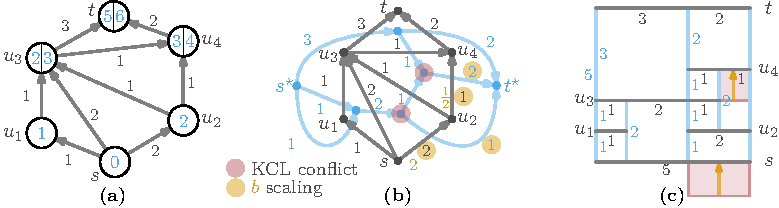
\includegraphics{networkAnalyzes/figures/AnalogiesSusceptanceScaling.pdf}
    % 
    \caption[Geometric interpretation of the susceptance scaling.]{%
    We use the example graph of~\textcite[p.18]{Fel13} that was already used
    in~\cref{ch:network-analysis} to show the geometric analogies for
    the~\gls{facts} placement. A~\gls{facts} placement basically represents a
    susceptance scaling. (a) Shows a feasible flow that is not a feasible
    electrical flow, since the \textcolor{THETA}{voltage
    angles~$\glssymbol{voltageangle} (\vertexa)$} at each
    vertex~$\vertexa\in\glssymbol{vertices}$ are not unique. This is illustrated
    at vertices~$\vertexa_3, \vertexa_4, \sink \in \glssymbol{vertices}$, where
    for example vertex~$\vertexa_3$ has two voltage angle labels~$
    \textcolor{THETA}{\glssymbol{voltageangle}_1(\vertexa_{3}) = 2}$ and~$
    \textcolor{THETA}{\glssymbol{voltageangle}_2(\vertexa_{3}) = 3}$. (b) The
    corresponding flows are shown in the \textcolor{PRIMALGRAPH}{primal
    graph~\glssymbol{graph}} and the \textcolor{DUALGRAPH}{dual
    graph~\glssymbol{dualgraph}} (see~\cref{ch:network-analysis} for more
    information). The flows on the two graphs do not map on the associated
    edges. A mapping of the primal flow would result in~\gls{kcl}
    conflicts~\tikzKclConflictMarker in the \textcolor{DUALGRAPH}{dual
    graph~\glssymbol{dualgraph}}. Applying the shown susceptance
    scaling~\tikzSusceptanceScaling results in a feasible electrical flow. 
    (c)~This is the geometric interpretation
    (see~\cref{ch:network-analyzes:rectangular-representation} for more
    information) of the \textcolor{SUSCEPTANCE}{susceptance scaling}, where each
    edge corresponds to a rectangle. A susceptance scaling is a scaling of a
    rectangle's aspect ratio by resizing it in one dimension (here we define it
    as a height scaling). The scaling reduces the height of the bottom right
    square of size~$\textcolor{DUALGRAPH}{2} \times \textcolor{PRIMALGRAPH}{2}$
    to a rectangle of size~$\textcolor{DUALGRAPH}{1} \times
    \textcolor{PRIMALGRAPH}{2}$ and the center right square of
    size~$\textcolor{DUALGRAPH}{1} \times \textcolor{PRIMALGRAPH}{1}$ to a
    rectangle of size~$\textcolor{DUALGRAPH}{2}
    \times \textcolor{PRIMALGRAPH}{1}$. The mentioned susceptance scaling
    removes the conflicts that are highlighted by the red areas.%
    }%
    %
    \label{ch:facts:analogies-susceptance-scaling}%
    % 
\end{figure}

Using the well-known~\gls{ieee} power systems test cases, we performed
simulation experiments related to two key questions, which take into account
that the~\gls{facts} needed for realizing our flow control units in reality
constitute a significant and expensive investment and hence their number should
be as small as possible.
%
\crefformat{enumi}{#2\textup{Question~#1}#3}%
\begin{enumerate}[(Q1)]%
    % 
    \item How many flow control units are required and where do they have to be
    placed in order to obtain a lower bound for the operating costs?
    \label{ch:facts:quest:main1}
    % 
    \item If the number of available flow control units is given, do we still
    see a positive effect on the operating costs and on the operability of the
    grid during peak periods of the~grid?
    \label{ch:facts:quest:main2}
    % 
\end{enumerate}%
% 
\begin{figure}[t]
    % 
    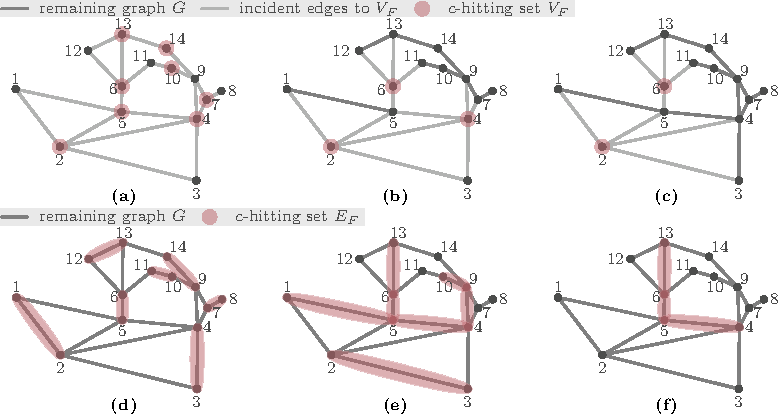
\includegraphics[page=1]{factsplacement/figures/FeedbackSetsVertexBased.pdf}
    % 
    \caption[Different vertex and edge hitting sets for the~\gls{ieee} 14
    system.]{%
    The~\gls{ieee} $14$ bus benchmark case is a graph~\glssymbol{graph} with
    $14$ vertices and~$20$ edges~\parencite{online:IEEEtestData}. The vertices
    (respectively edges) in the \textcolor{KITred70}{vertex hitting
    set~$\glssymbol{factsbus}^c$} (respectively \textcolor{KITred70}{edge
    hitting set~$\glssymbol{factsbranch}^c$}) are marked
    red~\textcolor{KITred70}{$\Large\bullet$}. Edges that are affected by a
    vertex hitting set have a \textcolor{KITblack50}{light gray color} and the
    remaining graph that we call \emph{native power grid}  has a
    \textcolor{KITblack70} {dark gray color}. (a)~The $1$-pumpkin hitting set
    (\ie, vertex cover) has~$\textcolor{KITred70}{\fmagnitude{\ffactsbus{1}} =
    8}$ vertices and the remaining graph~\glssymbol{graph} is empty. (b)~The
    $2$-pumpkin hitting set (\ie, feedback vertex set)
    has~$\textcolor{KITred70}{\fmagnitude{\ffactsbus{2}} = 3}$ vertices and the
    remaining graph is a forest. (c)~The $3$-pumpkin hitting set (\ie, diamond
    hitting set) has only~$\textcolor{KITred70}{\fmagnitude{\ffactsbus{3}} = 2}$
    vertices and the remaining graph is a cactus graph. (d)--(f) Represent the
    same results as (a)--(c), but on edges and the set is denoted by~$
    \glssymbol{factsbranch}^c$. We get the
    following sizes for the hitting set
    sizes~$\textcolor{KITred70}{\fmagnitude{\ffactsbranch{1}} = 7}$,
    $\textcolor{KITred70}{\fmagnitude{\ffactsbranch{2}} = 7}$, and
    $\textcolor{KITred70}{\fmagnitude{\ffactsbranch{3}} = 3}$.
    %
    }%
    % 
    \label{ch:facts:fig:feedback-sets-vertex-based}
    % 
\end{figure}
% 
In~\cref{ch:facts:sec:hybridmodel} we address the first question. In our
simulations we determine the minimum number of flow control vertices necessary
to achieve the same solution quality as in a power grid in which each vertex is
controllable and which clearly admits an upper bound on what can be achieved
with the network topology.
% 
% a globally optimal solution. 
% 
Interestingly, it turns out that a relatively small number of flow control units
are sufficient for this. In fact, we can prove a theorem stating a structural
graph-theoretic property, which, if met by the placement of flow control units,
implies the optimality of the power flow and serves as a theoretical explanation
of the observed behavior.
\Cref{ch:facts:sec:grid-control-when-approaching-capacity-limits} deals with the
second question of operating a power grid close to its capacity limits, which
becomes increasingly relevant as the consumption of electrical energy grows
faster than the grid capacities. Our experiments indicate that installing few
flow control units in a power grid is sufficient not only to achieve lower costs
compared to a solution of~\gls{opfp}, but also allows to operate the grid at
capacities for which no feasible solution of~\gls{opfp} exists any more.
%
%%%%%%%%%%%%%%%%%%%%%%%%%%%%%%%%%%%%%%%%%%%%%%%%%%%%%%%%%%%%%%%%%%%%%%%%%%%%%%%%
\section{Preliminaries}%
\label{ch:facts:sec:preliminaries}%
%%%%%%%%%%%%%%%%%%%%%%%%%%%%%%%%%%%%%%%%%%%%%%%%%%%%%%%%%%%%%%%%%%%%%%%%%%%%%%%%
% 
In this section we recall some basic notions from graph theory. Although, for
technical reasons, the graphs we use for modeling power grids are directed, when
considering the topology of the network, we always consider the underlying
undirected graph. Thus, in the following let~$
    % 
    \glssymbol{graph} 
    = (
    \glssymbol{vertices},
    \glssymbol{undirectededges})
    % 
$ be an undirected graph (see~\cref{ch:foundations:sec:graph-theory}).

The graph~\glssymbol{graph} is \emph{connected} if it contains a path between
any two vertices. A \emph{connected component} of~\glssymbol{graph} is a maximal
connected subgraph of~\glssymbol{graph} (maximal with respect to inclusion). A
\emph{cactus} is a graph where every edge is contained in at most one cycle. A
\emph{tree} is a connected graph that does not contain a cycle. A~\emph{forest}
consists of multiple connected components, where each connected component
constitutes a tree.

\begin{wrapfigure}{l}{4.7cm}%
    % 
    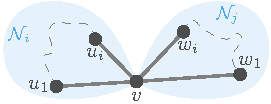
\includegraphics[scale=1,page=1]{factsplacement/figures/cutvertex.pdf}%
    % 
    \caption[A cutvertex decomposes the network.]{%
    A cutvertex~\vertex decomposes the network~\glssymbol{network} into at least
    two networks~$\glssymbol{network}_i$ and~$\glssymbol{network}_j$.
    %
    }%
    % 
    \label{ch:facts:fig:cutvertex}
    % 
\end{wrapfigure}%
%
A \emph{cut vertex} (also known as articulation point) is a vertex of a graph
whose removal increases the number of connected components
(see~\cref{ch:facts:fig:cutvertex}). Note from~\cref{ch:facts:fig:cutvertex}
that any path from vertex~$\vertexa_{i}$ to vertex~$\vertexc_{i}$ passes through
the cut vertex~\vertex. A \emph{biconnected component} is a maximal subgraph
that does not have a cut vertex. Biconnected components are also called
nonseparable graphs. Such nonseparable graphs with at least three edges have the
following properties: The nullity~$\nullity > 0$
(see~\cref{ch:network-analyzes:sec:mathematical-model:paragraph:property-incidence-matrix}),
$\degree(\vertex)\geq 2$ for all vertices~$\vertex\in\glssymbol{vertices}$, and
each edge lies on a cycle. The decomposition of a graph into its nonseparable
graphs is unique~\parencite[p.38]{Ses61}. Note that a biconnected component of a
forest is either \emph{trivial} in the sense that it consists of a single
vertex, or it consists of a single edge. Similarly, a biconnected component of a
cactus is trivial, a single edge, or a cycle. 

In the following we introduce two special hitting sets that are
the~\acrlong{vcp} (\gls{vcp}) and the~\acrlong{fvsp} (\gls{fvsp}), which we will
generalize in the next paragraph.
%
% Problem VC
\begingroup
    %%%%%%%%%%%%%%%%%%%%%%%%%%%%%%%%%%% Problem %%%%%%%%%%%%%%%%%%%%%%%%%%%%%%%%%%%%
\begin{problem}[framed]{\acrlong{vcp}~$\gls{vcp}(\glssymbol{graph},k)$}%
    % 
    Instance: & A graph~$\glssymbol{graph} = (\glssymbol{vertices},
    \glssymbol{undirectededges})$, and parameter~$k\in\naturals$.\\
    % 
    Question: & Is there a vertex cover~$\vc(\glssymbol{graph})$ of size at
    most~$k$ such that one endpoint of each edge~$
    \{\vertexa,\vertexc\}
    \in
    \glssymbol{undirectededges}
    % 
    $ belongs to a subset of~$
    \glssymbol{factsbus}^{c = 1} 
    \subseteq 
    \glssymbol{vertices}
    % 
    $ with~$
    \fmagnitude{\glssymbol{factsbus}^{c = 1}} 
    \leq 
    k
    $?
    % 
\end{problem}%
    \label{ch:facts:problem:vertex-cover}
\endgroup
%
% Problem FVC
\begingroup
    %
%%%%%%%%%%%%%%%%%%%%%%%%%%%%%%%%%%% Problem %%%%%%%%%%%%%%%%%%%%%%%%%%%%%%%%%%%%
\begin{problem}[framed]{\acrlong{fvsp}~$\gls{fvsp}(\glssymbol{graph},k)$}%
    % 
    Instance: & A graph~$\glssymbol{graph} = (\glssymbol{vertices},
    \glssymbol{undirectededges})$, and parameter~$k\in\naturals$.\\
    % 
    Question: & Is there a feedback vertex set~$\fvs(\glssymbol{graph})$ of
    size at most~$k$ such that at least one vertex of each
    cycle~$
    \glssymbol{cycle}
    \in
    \glssymbol{cycles}
    % 
    $ belongs to a subset of~$
    \glssymbol{factsbus}^{c = 2} 
    \subseteq 
    \glssymbol{vertices}
    % 
    $ with~$
    \fmagnitude{\glssymbol{factsbus}^{c = 2}} 
    \leq 
    k
    $?
    % 
\end{problem}%
    \label{ch:facts:problem:feedback-vertex-set}
\endgroup
% 

A \emph{vertex hitting set} of~$
\glssymbol{graph} 
= (
\glssymbol{vertices},
\glssymbol{edges})$ with respect to a class of graphs~$\mathcal G$ is a set of
vertices~$\glssymbol{factsbus}\subseteq\glssymbol{vertices}$ such
that~$\glssymbol{graph}-\glssymbol{factsbus} \in \mathcal G$. We will only be
interested in hitting sets with respect to forests and cacti. The former is also
called \emph{feedback vertex set}. Naturally, one is interested in finding a
set~$\glssymbol{factsbus}$ that is as small as possible. A generalization of
vertex

\begin{wrapfigure}{l}{4.7cm}%
    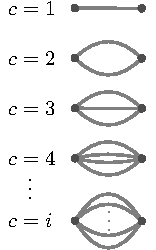
\includegraphics[scale=1,page=1]{factsplacement/figures/forbiddenMinors.pdf}%
    \caption{%
    Forbidden~$c$-pumpkin minors for different values of~$c$
    with~$c\in\naturals_{> 0}$.
    %
    }%
    \label{ch:facts:fig:forbidden-pumpkin-minors}%
\end{wrapfigure}%
% 
\noindent%
cover and feedback vertex set is called $c$-pumpkin hitting set. A
\emph{minor}~$\minor$ of a graph~\glssymbol{graph} is a graph that can be
obtained from~\glssymbol{graph} by deletion of vertices and edges or by
contraction of edges. A graph that has no c-pumpkin minor for~$c = 1$ is an
empty graph (\ie, vertex cover;
see~\cref{ch:facts:fig:feedback-sets-vertex-based}\screen{a}), for~$c = 2$ is a
forest (\ie, feedback vertex set;
see~\cref{ch:facts:fig:feedback-sets-vertex-based}\screen{b}), and for~$c = 3$
is a cactus (\ie, diamond hitting set;
see~\cref{ch:facts:fig:feedback-sets-vertex-based}\screen{c}). We call a subset
of vertices~$\glssymbol{factsbus}^c$ $c$-pumpkin hitting set if there is a
vertex
subset~$
\glssymbol{factsbus}^c
\subseteq
\glssymbol{vertices}(\glssymbol{graph})
$ such that~$
\glssymbol{graph}
-
\glssymbol{factsbus}^c
% 
$ consists of no~$c$-pumpkin minor
(see~\cref{ch:facts:fig:forbidden-pumpkin-minors} for different~$c$-minors). In
addition, we try to minimize the size of the $c$-pumpkin hitting set. The
general problem definition is given below.
%
%%%%%%%%%%%%%%%%%%%%%%%%%%%%%%%%%%% Problem %%%%%%%%%%%%%%%%%%%%%%%%%%%%%%%%%%%%
\begingroup
    %%%%%%%%%%%%%%%%%%%%%%%%%%%%%%%%%%% Problem %%%%%%%%%%%%%%%%%%%%%%%%%%%%%%%%%%%%
\begin{problem}[framed]{$c$-Pumkin Hitting Set Problem~$p$-$c$-Hit(%
$\glssymbol{graph},c,k$)~\parencite{Jor11a,Jor11b}}%
    Instance: & A graph~\glssymbol{graph}, parameter~$c\in\naturals_{>0}$, 
    and~$k\in\naturals$.\\
    % 
    Question: & Is there a~$c$-pumpkin hitting
    set~$\glssymbol{factsbus}^c\subseteq\glssymbol{vertices}$
    of size~$\fmagnitude{\glssymbol{factsbus}^c}\leq k$ such
    that~$\glssymbol{graph}-\glssymbol{factsbus}^c$
    consists of no~$c$-pumpkin minor?
    % 
\end{problem}%
% 
% 
% \begin{problem}[framed]{$c$-Pumkin Hitting Set Problem
% ($p$-$c$-Hit)~\parencite{Jor11a,Jor11b}}%
%     Instance: & A graph~\glssymbol{graph}, and parameter~$c\in\naturals_{>0}$
%     and~$k\in\naturals$.\\
%     % 
%     Objective: & Find a~$c$-pumpkin hitting set~$\factsbus^c\subseteq\vertices$
%     of size~$\fmagnitude{\factsbus^c}\leq k$ such that~$\graph-\factsbus^c$
%     consists of no~$c$-pumpkin minor.
% \end{problem}%
    \label{ch:facts:problem:c-pumkin-hitting-set}
\endgroup
% 
Note that the problem of finding a $c$-pumpkin hitting set is already~\NP-hard
for all~$c\geq 1$~\parencite{Jor11a,Jor11b}. Analogous to vertex hitting set, we
define the~\emph{edge hitting
set}~$\glssymbol{factsbranch}\subseteq\glssymbol{edges}$ such
that~$\glssymbol{graph} - \glssymbol{factsbranch}\in\mathcal\graph$ and a
$c$-pumpkin hitting set is denoted
by~$\glssymbol{factsbranch}^c\subseteq\glssymbol{edges}(
\glssymbol{graph})$.
% 
\paragraph{An Exact Model for (Special) Hitting Sets}
% 
In general a \emph{set system} (also known as hypergraph or range space) is a
tuple~$(\glssymbol{vertices},S)$, where~\glssymbol{vertices} is the set of
elements such as vertices and~$S$ is the set of subsets of~\glssymbol{vertices}
that is not necessarily a power set meaning~$\mathcal P(\glssymbol{vertices})$.
The latter would imply an exponential size of~$S$ with~$\fmagnitude{S} =
2^{\fmagnitude{\glssymbol{vertices}}}$. A \emph{hitting
set}~$\glssymbol{factsbus}\subseteq\glssymbol{vertices}$ is a set that has at
least one element in each subset of~$S$ meaning~$\glssymbol{factsbus}\cap
S_i\ne\emptyset$ for all~$S_i\in S$ with~$i\in\naturals$
(see~\cref{ch:facts:lp:hitting-set:eq:hitting-set-constraint}) and thus, a
hitting set highly depends on the definition of the set~$S$. One possibility to
define the set of subsets is~$
S 
= 
\bigcup_{\edge_i\in\glssymbol{edges}}
\{
S_i\cap\glssymbol{vertices}
\mid 
S_i 
=  
\edge_i,
\edge_i
=
\{\vertexa,\vertexb\}
\}$, which represent the set of subsets for vertex cover. The hitting set
problem is defined by~\cref{ch:facts:lp:hitting-set}.
% 
\begin{subequations}%
    \begin{align}
    & \underset{}{\text{minimize}}\hspace{-2cm} 
    & \sum_{\vertex\in\vertices} \switch(\vertex),& &
    \label{ch:facts:lp:hitting-set:eq:objective}
    \\
    & \text{subject to}\hspace{-3cm}& &
    \nonumber
    \\%
    &&\sum_{\vertex\in S_i} \switch(\vertex) &\geq 1
    &\forall S_i\in S,
    \label{ch:facts:lp:hitting-set:eq:hitting-set-constraint}
    %
\end{align}%
    \label{ch:facts:lp:hitting-set}%
\end{subequations}%
% 
where~$\glssymbol{switch}\colon\glssymbol{vertices}\to\{0,1\}$ is a decision
variable that is~$\glssymbol{switch}(\vertex) = 1$ if~\vertex is in the hitting
set~$\vertex\in\glssymbol{factsbus}$ and~$0$ otherwise. The latter represents
basically the integrality constraint that explains why this is an~\gls{ilp}. The
solution to the above defined~\gls{ilp} dependent on~$S$ is a hitting
set~$\ffactsbus{1}$ that is a~$1$-pumpkin hitting set (\ie, vertex
cover)~\parencite[p.60]{Cyg15}.

Now, we are interested in hitting sets such that the remaining graph has
no~$c$-pumpkin minor. Thus, we have to generalize the definition of~$S$ with
subsets~$S_i\in S$ such that~$S_i$ is a connected component (also known as
block) that is not~$c$-pumpkin minor free. We are looking for all such connected
components. This is quite similar to the~\acrlong{tsp} (\gls{tsp}) approach that
is generating subtour elimination constraints meaning if the tour does not have
the correct length then the tour represents a subtour that is excluded from the
solution set. However, we add a restriction to the structure of~$S_i$ that is a
connected component that has at least one~$c$-pumpkin minor. Thus, in each
solver callback we add new sets~$S_i$ with~$ S_i
\subseteq
\glssymbol{vertices}
\setminus
\bigcup_{\vertex\in\glssymbol{vertices}}
\{\vertex
\mid
\glssymbol{switch}(\vertex)=1
\}$. For~$c$-pumpkins with~$c = 2$ or~$c = 3$ we use block-cut trees to identify
the set of maximum biconnected components and check by the ratio of the number
of vertices to the number of edges whether each new connected component~$\block$
is large enough. This means that for~$c = 2$, we have~$\fmagnitude{
\glssymbol{vertices} (\block)}-1 <
\fmagnitude{\glssymbol{edges}(\block)}$ that excludes trees and for~$c = 3$ we
have~$
\fmagnitude{\glssymbol{vertices}(\block)} 
<
\fmagnitude{\glssymbol{edges}(\block)}
$ that excludes simple cycles. This can be extend to any~$c\in\naturals$
(see~\cref{ch:facts:fig:forbidden-pumpkin-minors}).
%
% \begin{subequations}
%     \begin{align}
    & \underset{}{\text{minimize}}\hspace{-2cm} 
    & \sum_{\vertex\in\vertices} \switch(\vertex),&
    % 
    \label{ch:facts:lp:pumpkin-hitting-set:eq:objective}
\\
    & \text{subject to}\hspace{-3cm}& &
    \nonumber
\\%
    & & \sum_{\vertex\in S_i} \switch(\vertex) &\geq 1
    & \forall S_i\in S,
    % 
    \label{ch:facts:lp:pumpkin-hitting-set:eq:hitting-set-constraint}
\\
    & & \sum_{\vertex\in S_i} \fmagnitude{\edges(\block)} &\geq 
    \fmagnitude{\vertices(\block)}-1+c
    & \block\subsetneq S, \block\neq\emptyset,
    % 
    \label{ch:facts:lp:pumpkin-hitting-set:eq:subtour-exclusion}
    %
\end{align}
%     \label{ch:facts:lp:pumpkin-hitting-set}
% \end{subequations}
% 
The substructure exclusion leads to exponentially many constraints. Thus, a
common way to solve this~\gls{ilp} is by using techniques such as column
generation.
% 
%
%%%%%%%%%%%%%%%%%%%%%%%%%%%%%%%%%%%%%%%%%%%%%%%%%%%%%%%%%%%%%%%%%%%%%%%%%%%%%%%%
\section[A Hybrid Mathematical Model for the Placement of Continuous Control Units]{
A Hybrid Mathematical Model for the \protect\linebreak{Placement of Continuous Control Units}} 
% 
\label{ch:facts:sec:model} 
%%%%%%%%%%%%%%%%%%%%%%%%%%%%%%%%%%%%%%%%%%%%%%%%%%%%%%%%%%%%%%%%%%%%%%%%%%%%%%%%
%
In this section we introduce three graph-theoretic flow models for optimal power
flows. We propose a~\emph{hybrid model} that combines the flow model and the
electrical flow model in order to handle power grids with flow control units.
Our models are based on the~\gls{dc} power grid model~\parencite{Ham07,
Zimmerman2011a,sja-dcpfr-09}, which is commonly used as an approximation
of~\gls{ac} grids~\parencite{Pur05,ocs-acdc-04}. An overview of the
simplifications is given
in~\cref{ch:foundations:sec:power-flow-analyses:subsec:Lin-DC-Model}. We model a
power grid~\glssymbol{network} as a graph~$\glssymbol{graph} =
(\glssymbol{vertices}, \glssymbol{edges})$, where~\glssymbol{vertices} is the
set of vertices and~$\glssymbol{edges}\subseteq \binom{\glssymbol{vertices}}{2}$
is the set of edges. The underlying power grid is an undirected graph. We model
the undirected graph using a directed graph by replacing the undirected edges~$
\{\vertexa,\vertexb\}$ by two directed
edges~$(\vertexa,\vertexb),(\vertexb,\vertexa)\in\glssymbol{edges}$ that are
directed to either vertices of the original edge. However, in some cases we
neglect for the notational convenience the orientation and use the undirected
edge that is denoted by~$\undirectededge\in\glssymbol{undirectededges}$,
where~\undirectededge is the undirected edge of~\edge. The vertices represent
the buses, some of which may be special generator and consumer vertices, and the
edges represent the branches, which may be transmission lines between the
incident vertices or transformers. There is a
subset~$\glssymbol{generators}\subseteq\glssymbol{vertices}$ of the vertices
that represent generator vertices. We define the
functions~$\glssymbol{realpowergenerationmin},\glssymbol{realpowergenerationmax}\colon\glssymbol{generators}\to\posreals$
that represent the minimum and maximum supply for each generator, respectively.
In this chapter, we assume that the lower generation bound is zero
meaning~$\glssymbol{realpowergenerationmin}\equiv 0$. Further, there is a
subset~$\glssymbol{consumers} \subseteq \glssymbol{vertices} \setminus
\glssymbol{generators}$ of consumer vertices. We define the
functions~$
\glssymbol{realpowerdemandmin},
\glssymbol{realpowerdemandmax}
\colon
\glssymbol{consumers}
\to
\reals
\cup
\{\infty\}$ that represents the minimum and maximum real power demand,
respectively. We assume that the demands are fixed
meaning~$\glssymbol{realpowerdemandmin}(\vertexa) =
\glssymbol{realpowerdemandmax}(\vertexa) =
\glssymbol{realpowerdemand}(\vertexa)$ for each consumer~$\vertexa \in
\glssymbol{consumers}$. Without loss of generality, we assume
that~$\glssymbol{generators}\cap\glssymbol{consumers} = \emptyset$.
% 
%%%%%%%%%%%%%%%%%%%%%%%%%%%%%%%%%%%%%%%%%%%%%%%%%%%%%%%%%%%%%%%%%%%%%%%%%%%%%%%%
\subsection{The Objective Function}
\label{ch:facts:sec:model:objective-function}
%%%%%%%%%%%%%%%%%%%%%%%%%%%%%%%%%%%%%%%%%%%%%%%%%%%%%%%%%%%%%%%%%%%%%%%%%%%%%%%%
% 
Each generator~$\vertexa\in\glssymbol{generators}$ is equipped with a convex cost
function~$\fcost{\vertexa}\colon\reals\to\posreals$ with~$\fcost{\vertexa} > 0$
that is assumed to be piecewise linear
(see~\cref{ch:facts:eq:generatorcostfunction}).
% 
\begin{equation}
    \fcost{\vertexa}(x) 
    = 
    \max\{a_i x + c_i \mid(a_i, c_i)\in \fsetPiecwisefct{\vertexa}\},
    % 
    \label{ch:facts:eq:generatorcostfunction}
\end{equation}
% 
where~$\fsetPiecwisefct{\vertexa}$ is the set of all piecewise linear functions
of~$\fcost{\vertexa}$ and~$a_i \leq a_{i+1}$ for~$i\in\naturals$. 

Each edge~$\edge \in \glssymbol{edges}$ has a thermal line limit that is modeled by a
capacity function~$\glssymbol{capacity} \colon \glssymbol{edges} \to \reals$ restricting the real
power. Further, each edge causes a certain loss of power depending on the
physical edge parameters and the actual power flow on that edge. These losses
are again approximated as a convex, piecewise linear
function~$\floss{\edge}\colon\reals\to\posreals$ for each edge~$\edge \in
\glssymbol{edges}$ (see~\cref{ch:facts:eq:losscostfunction}).
% 
\begin{equation}
    \floss{\edge}(x) = \max\{a_i x + c_i \mid(a_i, c_i)\in \fsetPiecwisefct{\edge}\},
    \label{ch:facts:eq:losscostfunction} 
\end{equation}
% 
where~$\fsetPiecwisefct{\edge}$ is the set of all piecewise linear functions
of~$\ell_\edge$ and~$a_i \leq a_{i+1}$ for~$i\in\naturals$.

A~\emph{flow}~\glssymbol{flow} in a power grid~\glssymbol{network} is a
function~$\glssymbol{flow} \colon
\glssymbol{vertices} \times \glssymbol{vertices} \to \reals$ that complies with the skew symmetry
property~$\glssymbol{flow}(\vertexa,\vertexb) = -\glssymbol{flow}(\vertexb,\vertexa)$ for
all~$\vertexa, \vertexb \in \glssymbol{vertices}$.
% 
For every vertex~\vertexa in~$\glssymbol{vertices}(\glssymbol{graph})$, we
define its \emph{net out-flow} $\glssymbol{netflow}(\vertexa) \coloneq
\sum_{\{\vertexa,\vertexb\}
\in\undirectededges}
\glssymbol{flow}(\vertexa,\vertexb)$.
% 
For a flow~\glssymbol{flow}, we further define two types of cost functions. The total
\emph{generator cost} is a function~$\gencost\colon\reals\to\posreals$ that is
defined in~\cref{ch:facts:eq:total-generator-cost} and the total \emph{line
loss} is a function~$\losscost\colon\reals\to\posreals$ that is defined
in~\cref{ch:facts:eq:total-loss-cost}.
% 
\begin{align}
    \gencost(\glssymbol{flow}) 
    &= 
    \sum_{\vertexa \in \glssymbol{generators}} \fcost{\vertexa} ( \glssymbol{netflow}(\vertexa) ),
    % 
    \label{ch:facts:eq:total-generator-cost}
    \\
    % 
    \losscost(\glssymbol{flow}) 
    &= 
    \sum_{(\vertexa,\vertexb) \in \glssymbol{edges}} 
    \floss{(\vertexa,\vertexb)}(\fmagnitude{\glssymbol{flow}(\vertexa,\vertexb)})\,.
    % 
    \label{ch:facts:eq:total-loss-cost}
    % 
\end{align}
% 
To obtain the overall cost for a flow~\glssymbol{flow}, we weight these two
terms with~$\lambda\in [0,1]$ such that the objective function represents a
multi-criteria objective (see~\cref{ch:facts:eq:objective}) weighted
with~$\lambda$.
% 
\begin{equation}
    \totalgenlosscost(\glssymbol{flow}) = \lambda \cdot \gencost(\glssymbol{flow}) + (1-\lambda) \cdot
    \losscost(\glssymbol{flow}).
    \label{ch:facts:eq:objective}
\end{equation}
% 
Our goal is to minimize this objective function~\totalgenlosscost in different
models.
%
%%%%%%%%%%%%%%%%%%%%%%%%%%%%%%%%%%%%%%%%%%%%%%%%%%%%%%%%%%%%%%%%%%%%%%%%%%%%%%%%
\subsection{Power Flow Models}%
\label{ch:facts:sec:power-flow-models}%
%%%%%%%%%%%%%%%%%%%%%%%%%%%%%%%%%%%%%%%%%%%%%%%%%%%%%%%%%%%%%%%%%%%%%%%%%%%%%%%%
%
The most basic model is the \emph{flow model}, where~\glssymbol{flow} has to satisfy the
constraints given in
the~\crefrange{ch:facts:eq:conservation}{ch:facts:eq:capacity}.
% 
We call a flow satisfying these constraints \emph{feasible}.
\Cref{ch:facts:eq:capacity} models the thermal line limits or real power
capacities of all edges and is called \emph{capacity constraint}.
\Cref{ch:facts:eq:conservation} models the zero net out-flow for intermediate
vertices, \ie, vertices that are neither generators nor consumers.
\Cref{ch:facts:eq:consumer} models that all consumer demands are satisfied and
is called \emph{demand constraint}. Finally, \cref{ch:facts:eq:generator}
models that all generators respect their production limits and is called
\emph{generator constraint}.
The~\crefrange{ch:facts:eq:conservation}{ch:facts:eq:generator} are called
\emph{flow conservation constraints}.
% 
\begin{align}
    % 
    \glssymbol{netflow} ( \vertex ) & =  0 & \vertex \in \glssymbol{vertices} \setminus 
    ( \glssymbol{generators} \cup \glssymbol{consumers} ),
    \label{ch:facts:eq:conservation}\\
    % 
    \glssymbol{netflow} ( \vertex ) & =   -\glssymbol{realpowerdemand}(\vertex) & \vertex \in
    \glssymbol{consumers},
    \label{ch:facts:eq:consumer}\\
    % 
    0 \le \glssymbol{netflow} ( \vertex ) & \le \glssymbol{realpowergenerationmax}(\vertex) & 
    \vertex \in \glssymbol{generators},
    \label{ch:facts:eq:generator}\\
    % 
    \fmagnitude{\glssymbol{flow} ( \vertexa, \vertexb )} 
    & 
    \leq 
    \glssymbol{capacity}( \vertexa, \vertexb )
    &  
    \forall (\vertexa, \vertexb) \in \glssymbol{edges}.
    \label{ch:facts:eq:capacity}
\end{align}
% 
The flow model (\ie, \crefrange{ch:facts:eq:conservation}{ch:facts:eq:capacity})
neglects some physical properties of electrical flows, in particular Kirchhoff's
voltage law.  Thus, the computed power flows can only be applied to power grids
where every vertex is a control vertex.  In contrast, the~\emph{electrical flow
model}, \eg, according to~\textcite{Zimmerman2011a}, models the power flow using
the same set of constraints as the flow model, but additionally requires the
existence of a suitable voltage angle assignment~$\glssymbol{voltageangle}
\colon \glssymbol{vertices} \to
\reals$ such that for each edge~$
\{ \vertexa, \vertexb \}\in\glssymbol{undirectededges}$ the power flow specific
constraint
holds (see~\cref{ch:facts:eq:electricalflowintro}). The power flow constraint
basically represents~\KVL (\kvl) that is combined with Ohm's law. More
details can be found in~\cref{ch:network-analysis}.
% 
\begin{equation}
    \glssymbol{flow}(\vertexa,\vertexb) 
    = 
    \glssymbol{susceptance}(\vertexa,\vertexb) 
    (
        \glssymbol{voltageangle}(\vertexb)
        - 
        \glssymbol{voltageangle}(\vertexa)
    ),
  % 
  \label{ch:facts:eq:electricalflowintro}
  % 
\end{equation}
% 
where the \emph{susceptance}~$\glssymbol{susceptance}(\vertexa,\vertexb)$ is a
function~$\glssymbol{susceptance}\colon\glssymbol{edges}\to\reals$. This is
equivalent to restricting the model to feasible flows that also satisfy
the~\gls{kvl}, or, in other words, no flow control units are used. This yields a
model that matches the situation in the traditional power grid existing today.
We call a feasible flow~\glssymbol{flow}~a~\emph{feasible electrical flow} if
there exists a voltage angle assignment~$\glssymbol{voltageangle}$
satisfying~\cref{ch:facts:eq:electricalflowintro}. We are now able to give a
complete definition of the power grid by the tuple~$\glssymbol{network} = (
\glssymbol{graph}=(\glssymbol{vertices},\glssymbol{edges}),
\glssymbol{generators},
\glssymbol{consumers},
\glssymbol{capacity},
\glssymbol{susceptance}, 
\fcost{\vertexa\in\glssymbol{generators}},
\floss{\edge\in\glssymbol{edges}},
\glssymbol{realpowergenerationmin}, 
\glssymbol{realpowergenerationmax}, 
\glssymbol{realpowerdemand})$.

Recall from the introduction that flow control vertices (\gls{fcv}s) and flow
control edges (\gls{fce}s) can be technically realized by~\mbox{\gls{upfc}s},
which are~\gls{facts}. Ideal~\gls{facts} as introduced
by~\textcite{julieGriffin} are often used to simplify the modeling
of~\gls{facts} by using a linear model and assuming a complete and independent
control of the real and reactive power. Our flow control units are
ideal~\gls{facts} that control the power flow to all incident edges in terms of
\gls{fcv}s and the power flow on that particular edge in terms of~\gls{fce}s.
The flow model---in contrast to the electrical model---assumes flow control
units at each vertex or each edge, whereas the electrical model assumes no
immediate control of the power flow. Instead, the grid is balanced by changing
the generator outputs only.  In the following, we propose a~\emph{hybrid model}
that combines the flow model and the electrical flow model in order to handle
power grids with flow control vertices (resp. edges) at a subset of selected
vertices (resp. edges).
%
%%%%%%%%%%%%%%%%%%%%%%%%%%%%%%%%%%%%%%%%%%%%%%%%%%%%%%%%%%%%%%%%%%%%%%%%%%%%%%%%
\subsection{Flow Control Units on Vertices}%
\label{ch:facts:sec:flow-control-units-on-vertices}%
%%%%%%%%%%%%%%%%%%%%%%%%%%%%%%%%%%%%%%%%%%%%%%%%%%%%%%%%%%%%%%%%%%%%%%%%%%%%%%%%
% 
In this section, we focus on continuous flow control units that are placed on
vertices. As mentioned above, we call them flow control vertices (in
short~\gls{fcv}s). Let~$\glssymbol{factsbus} \subseteq\glssymbol{vertices}$ be a
subset of vertices of~\glssymbol{graph}.  We denote
by~$\glssymbol{graph}_{\glssymbol{factsbus}}$ the power network obtained
from~\glssymbol{graph} by considering all vertices in~\glssymbol{factsbus} as
flow control vertices.  We call any subgraph~$
\glssymbol{graph}' 
=
\glssymbol{graph} [ \glssymbol{vertices}' ] $ induced by a
subset~$
\glssymbol{vertices}'
\subseteq
\glssymbol{vertices}
\setminus
\glssymbol{factsbus}$ of the vertices without controllers a \emph{native power
grid} of~\glssymbol{graph}.  A flow~\glssymbol{flow} on~\glssymbol{graph} is a
\emph{feasible electrical flow} for a native power
grid~$\glssymbol{graph}'\subseteq\glssymbol{graph}$ if there exists a voltage
angle assignment~$\glssymbol{voltageangle}\colon\glssymbol{vertices}\to\reals$
such that every edge in~$\glssymbol{graph}'$
satisfies~\cref{ch:facts:eq:electricalflowintro}. In this case we
call~\glssymbol{voltageangle} a \emph{feasible (voltage) angle assignment}
for~$\glssymbol{graph}'$.

A feasible flow~\glssymbol{flow} is a \emph{feasible electrical flow
for~$\glssymbol{graph}_{\glssymbol{factsbus}}$} if and only if~\glssymbol{flow}
is a feasible electrical flow for the \emph{maximal native power grid}~$
\glssymbol{graph}
-
\glssymbol{factsbus} 
=
\glssymbol{graph} 
[ 
\glssymbol{vertices}
\setminus
\glssymbol{factsbus} 
] 
$. Intuitively, this models the fact that a power flow
in~$\glssymbol{graph}_{\glssymbol{factsbus}}$ must be a feasible flow and that
it satisfies the Kirchhoff's voltage law in the maximum native power grid.

Obviously, if~$\glssymbol{factsbus}\subseteq\glssymbol{factsbus}'$
and~\glssymbol{flow} is a feasible electrical flow
for~$\glssymbol{graph}_{\glssymbol{factsbus}}$, then~\glssymbol{flow} is also a
feasible electrical flow for~$\glssymbol{graph}_{\glssymbol{factsbus}'}$. Hence
the minimum value of the cost~$\totalgenlosscost$ does not increase when adding
more flow control buses.

We note that each of the models can easily be expressed as a~\acrlong{lp}
(\gls{lp}), and thus in all three models an optimal solution can be
computed efficiently~\parencite{Baz04}; see~\cref{ch:facts:lp:FCV-and-FCE}.
However, the flow model can be reduced to a special minimum cost network flow
problem, for which efficient exact optimization algorithms
exist~\parencite{Goldberg19971}. We describe this reduction in
the~\cref{ch:facts:sec:model-mincost-flow}.

We present the problem formulation as an~\acrlong{ilp} (\gls{ilp}) formulation
(see~\cref{ch:facts:lp:FCV-and-FCE}). Though~\cref{ch:facts:lp:FCV-and-FCE} has
only linear constraints---which would imply that we have an~\gls{ilp}---the
objective function has two piecewise linear cost functions, where the decision
of which piece we select is done by an integer variable. Thus, the whole program
is an~\gls{ilp}. In the~\gls{ilp}, we minimize the generation costs~$\gencost$
and losses~$\losscost$ shown in~\cref{ch:facts:lp:FCV:eq:objective} under flow
and electrical constraints. The main flow constraints comprise the conservation
of flow (\cref{ch:facts:lp:FCV:eq:conservation}), demand and generator
constraints (\cref{ch:facts:lp:FCV:eq:demand,ch:facts:lp:FCV:eq:generator}), and
capacity constraints (\cref{ch:facts:lp:FCV:eq:capacity}). Whereas the
electrical constraints describe the electrical feasibility for the native power
grid shown in~\cref{ch:facts:lp:FCV:eq:electricalfeasible}. Recall that each
consumer~$\vertexa\in\glssymbol{consumers}$ has a fixed power
demand~$\glssymbol{realpowerdemand}(\vertexa)\in\reals$
and~$\glssymbol{factsbus}\subseteq\glssymbol{vertices}$ is the set of flow
control vertices.
% 
\begin{subequations}
    \begin{align}
    & \underset{\glssymbol{flow}}{\text{minimize}}\hspace{-2cm} 
    & \totalgenlosscost(\glssymbol{flow})\,=\,
    & \lambda 
    \cdot
    \gencost(\glssymbol{flow}) 
    + 
    (1-\lambda)
    \cdot 
    \losscost(\glssymbol{flow})
    \label{ch:facts:lp:FCV:eq:objective}
\\
% 
& \text{subject to}\hspace{-3cm}&
\nonumber
\\
    & & 
    % \sum_{
    %     \{\vertexb,\vertexa\} 
    %     \in 
    %     \glssymbol{undirectededges}
    % } 
    \glssymbol{netflow}(\vertexb)\,=\,
    &  0 
    &
    & & & 
    \forall
    \vertexb 
    \in 
    \glssymbol{vertices} 
    \setminus (
    \glssymbol{generators} 
    \cup 
    \glssymbol{consumers}
    )
    % 
    \label{ch:facts:lp:FCV:eq:conservation}
\\
    & & \glssymbol{flow}(\vertexa, \vertexb )\,=\,
    & \glssymbol{susceptance}(\vertexa, \vertexb) 
    (\glssymbol{voltageangle}(\vertexa) 
    - 
    \glssymbol{voltageangle}(\vertexb))
    & & & & 
    % 
    \hspace{-1cm}
    \begin{cases}
        \forall \{\vertexa,\vertexb\}\in~\glssymbol{edges} \text{ s.t. }
        \vertexa,\vertexb
        \notin
        \glssymbol{factsbus}~\text{for~\gls{fcv}s}
        \\
        \forall \{\vertexa,\vertexb\} 
        \in 
        \glssymbol{edges} 
        \setminus
        \glssymbol{factsbranch}
        \hspace{1.35cm}~\text{for~\gls{fce}s}
    \end{cases}
    % 
    \label{ch:facts:lp:FCV:eq:electricalfeasible}
\\
    & & 
    % \sum_{\{\vertexb,\vertexa\} 
    % \in 
    % \glssymbol{edges}} 
    \hspace{1.2cm}
    \glssymbol{netflow}(\vertexb)\,=\,
    &  
    -\glssymbol{realpowerdemand}(\vertexb) 
    & & & & 
    \vertexb \in \glssymbol{consumers}
    % 
    \label{ch:facts:lp:FCV:eq:demand}
\\ 
    & & 0\,\leq\,
    & 
    % \sum_{\{\vertexb,\vertexa\}\in \glssymbol{edges}} 
    \glssymbol{netflow}(\vertexb)
    \,\le\,
    \glssymbol{realpowergenerationmax}(\vertexb) 
    & & & & 
    \vertexb 
    \in 
    \glssymbol{generators} 
    \label{ch:facts:lp:FCV:eq:generator}
\\
    & & %-\glssymbol{capacity}(\edge)\,\leq\,
    & 
    \fmagnitude{\glssymbol{flow} ( \vertexa, \vertexb )}\,\leq\, 
    \glssymbol{capacity}(\vertexa, \vertexb)
    & & & &
    \forall (\vertexa, \vertexb) \in \glssymbol{edges}.
    % 
    \label{ch:facts:lp:FCV:eq:capacity}
% 
\end{align}
    \label{ch:facts:lp:FCV-and-FCE}
\end{subequations}
% 
However, note that the~\gls{ilp} represents the hybrid model, which solves the
feasibility problem only. A proper problem definition and an overview of related
problems will be given in~\cref{ch:facts:sec:complexity}. In addition, different
possibilities to place control units are given
in~\cref{ch:facts:sec:hybridmodel}. The latter will make extensive use of the
above formulation.
% 
%%%%%%%%%%%%%%%%%%%%%%%%%%%%%%%%%%%%%%%%%%%%%%%%%%%%%%%%%%%%%%%%%%%%%%%%%%%%%%%%
\subsection{Flow Control Units on Edges}%
\label{ch:facts:sec:flow-control-units-on-edges}%
%%%%%%%%%%%%%%%%%%%%%%%%%%%%%%%%%%%%%%%%%%%%%%%%%%%%%%%%%%%%%%%%%%%%%%%%%%%%%%%%
% 
We define analogously to the set of \emph{flow control vertices} (\gls{fcv}s)
the set of \emph{flow control edges} (\gls{fce}s) that is denoted
by~$\glssymbol{factsbranch}\subseteq\glssymbol{edges}$. \gls{fce}s are edges
with ideal~\gls{facts} controlling flow on them. We denote
by~$\glssymbol{graph}_{\glssymbol{factsbranch}}$ the subgraph
of~\glssymbol{graph} that contains all edges of~\glssymbol{factsbranch} and
their incident vertices.

In the standard \emph{flow model} the flow on all edges can be manipulated, \ie,
it is like having a~\gls{facts} on every edge in a power grid. In case of
\gls{fce}s this means~$\glssymbol{factsbranch} = \glssymbol{edges}$. The
standard flow model asks to find a flow, \ie, it
neglects~\cref{ch:facts:eq:electricalflowintro}. In the \emph{\gls{dc} flow
model}~\parencite{Zimmerman2011a} the flow on edges cannot be controlled, which
translates to~$\glssymbol{factsbranch} = \emptyset$ in case of \gls{fce}s. The
\emph{\gls{dc} flow model} requires to find a feasible electrical flow, \ie,
\cref{ch:facts:eq:electricalflowintro} satisfied for all
edges~$\edge\in\glssymbol{edges}\setminus\glssymbol{factsbranch}$. The
\emph{hybrid model} is formalized in~\cref{ch:facts:lp:FCV-and-FCE} as
an~\gls{lp}, the flow model and the~\gls{dc} flow model are combined and it is
required to find a flow on~$\glssymbol{graph}_{\glssymbol{factsbus}}$ such
that~\cref{ch:facts:eq:electricalflowintro} holds only for edges that are not
in~\glssymbol{factsbranch}.

Since an \emph{ideal~\gls{facts}}~\parencite{julieGriffin} is technically
realized on transmission lines, it is more realistic to consider \gls{fce}s
instead of \gls{fcv}s. However, we can easily translate the described models
designed for \gls{fcv}s to models on \gls{fce}s by simply
replacing~\glssymbol{factsbus} by~\glssymbol{factsbranch}
and~$\glssymbol{graph}_{\glssymbol{factsbus}}$
by~$\glssymbol{graph}_{\glssymbol{factsbranch}}$ and vice versa
(see~\cref{ch:facts:lp:FCV:eq:electricalfeasible}).

Recall that the~\gls{edp} is the problem of generating the required amount of
power while obtaining minimum operation cost and meeting the constraints
in~\crefrange{ch:facts:eq:conservation}{ch:facts:eq:generator}. The objective
function~$\totalgenlosscost(\glssymbol{flow})$ describing the operation cost is
a weighted function of generator costs~$\gencost(\glssymbol{flow})$ and
transmission line losses~$\losscost(\glssymbol{flow})$, where~$\lambda\in[0,1]$
is the weight factor
(see~\cref{ch:facts:eq:objective,ch:facts:lp:FCV:eq:objective}). The overall
optimization problem is given in~\cref{ch:facts:lp:FCV-and-FCE} as an~\gls{lp}.
% 
%%%%%%%%%%%%%%%%%%%%%%%%%%%%%%%%%%%%%%%%%%%%%%%%%%%%%%%%%%%%%%%%%%%%%%%%%%%%%%%%
\subsection{Reduction to MinCostFlow}
\label{ch:facts:sec:model-mincost-flow}
%%%%%%%%%%%%%%%%%%%%%%%%%%%%%%%%%%%%%%%%%%%%%%%%%%%%%%%%%%%%%%%%%%%%%%%%%%%%%%%%
%
Let~$
\glssymbol{network} 
= (
\glssymbol{graph} = (\glssymbol{vertices},\glssymbol{edges}), 
\source, 
\sink, 
\glssymbol{capacity},
\edgeCost)
$ be a \emph{\source-\sink flow network} consisting of a directed
\mbox{(multi-)} graph~\glssymbol{graph}, two dedicated source and sink
vertices~$\source, \sink \in \glssymbol{vertices}$, edge capacities $
\glssymbol{capacity}\colon
\glssymbol{edges} 
\to 
\posreals$, and edge costs~$
\edgeCost 
\colon 
\glssymbol{edges} 
\to 
\posreals$. A \emph{flow}~\glssymbol{flow} in~\glssymbol{network} is a
function~$\glssymbol{flow} \colon \glssymbol{edges} \to
\posreals$ and it is called~\emph{feasible} if it satisfies the capacity
constraint in~\cref{ch:facts:eq:capacity} and a flow conservation constraint
similar to~\cref{ch:facts:eq:conservation} that is given
in~\cref{ch:facts:sec:min-cost:flow-conservation}.
% 
\begin{equation}%\label{ch:facts:eq:flow}
    % 
    \sum_{(\vertexa, \vertexb) \in \glssymbol{edges}} 
    % 
    \glssymbol{flow} ( \vertexa, \vertexb ) 
    - 
    \sum_{(\vertexb, \vertexa) \in \glssymbol{edges}} 
    \glssymbol{flow}(\vertexb, \vertexa) 
    = 
    0 
    \qquad \forall
    \vertexb \in \glssymbol{vertices} 
    \setminus 
    \{ \source, \sink \}.
    % 
    \label{ch:facts:sec:min-cost:flow-conservation}
    % 
\end{equation}
% 
The \emph{flow value}~$\glssymbol{flowvalue}(\glssymbol{network})$ of a
flow~\glssymbol{flow} is the total flow from~\source to~\sink, \ie,
$
\glssymbol{flowvalue}(\glssymbol{network}) 
=
\sum_{(\vertexa, \sink) \in \glssymbol{edges}} 
\glssymbol{flow}(\vertexa, \sink) 
= 
\sum_{ (\source, \vertexa) \in \glssymbol{edges}} 
\glssymbol{flow} (\source, \vertexa)
$. A feasible flow~\glssymbol{flow} with maximum value is called a \emph{maximum
flow} in~\glssymbol{network} and denoted by~$\mf(\glssymbol{network})$. For a
given flow value~$x$ the \emph{min-cost~\source-\sink flow problem} is to find a
feasible flow~\glssymbol{flow} of
value~$\glssymbol{flowvalue}(\glssymbol{network}) = x$ such that the
cost~$
c_{\glssymbol{network}}(\glssymbol{flow}) 
= 
\sum_{\edge \in \glssymbol{edges}}
\edgeCost(\edge) 
\cdot 
\glssymbol{flow}(\edge)$ is minimized.
%
% Problem
\begingroup
    %%%%%%%%%%%%%%%%%%%%%%%%%%%%%%%%%%% Problem %%%%%%%%%%%%%%%%%%%%%%%%%%%%%%%%%%%%
\begin{problem}[framed]{Min-cost s-t Flow Problem}%
    Instance: & A network~\glssymbol{network}, parameter~$x\in\reals$, 
    and~$k\in\posreals$.\\
    % 
    Question: & Is there a feasible flow~\glssymbol{flow} of
    value~$\glssymbol{flowvalue}(\glssymbol{network}) = x$ such
    that~$c_{\glssymbol{network}}(\glssymbol{flow})\leq k$?
    % 
    \label{problems:facts:min-cost-s-t-flow-problem}
    % 
\end{problem}%
% 
% \begin{problem}[framed]{Min-cost s-t Flow Problem}%
%    Instance: & A network~\glssymbol{network}, parameter~$x\in\reals$, 
%    and~$k\in\posreals$.\\
%    % 
%    Objective: & Find a feasible flow~\glssymbol{flow} of value~$\glssymbol{flow}value(\glssymbol{network}) = x$
%    such that~$c_{\glssymbol{network}}(\glssymbol{flow})\leq k$.
% \end{problem}%
    \label{ch:facts:problem:min-cost-s-t-flow-problem-decision-problem}
\endgroup
% 
In~\cref{ch:foundations:sec:graph-theoretical-flows}, we discussed some
approaches to tackle the problem. In order to transform the
graph~$\glssymbol{graph} = ( \glssymbol{vertices}, \glssymbol{edges} )$ of a
power grid into an~\source-\sink flow network~\glssymbol{network}, we first add
a new source vertex~\source and a new sink vertex~\sink to~\glssymbol{vertices}.
Each generator~$\vertexa \in \glssymbol{generators}$ is connected by a directed
edge~$(\source,\vertexa)$ with capacity~$\glssymbol{capacity} (\source,\vertexa)
= \glssymbol{realpowergenerationmax}(\vertexa)$ to the source~\source. Each
consumer~$\vertexa \in \glssymbol{consumers}$ is connected by a directed edge~$
(\vertexa,\sink)$ with capacity~$\glssymbol{capacity} (\vertexa,\sink) =
\glssymbol{realpowerdemand}(\vertexa)$ to the sink~\sink. Further, we replace
each original undirected edge~$\{ \vertexa,\vertexb \} \in \glssymbol{edges}$ by
two directed edges~$(\vertexa,\vertexb)$ and~$(\vertexb,\vertexa)$, whose
capacities~$\glssymbol{capacity}(\vertexa, \vertexb) =
\glssymbol{capacity}(\vertexb, \vertexa)$ are given by their common thermal
limit~$\glssymbol{capacity}( \{ \vertexa, \vertexb \} )$. Recall from the
introduction of~\cref{ch:facts:sec:model} that this represents a bidirected
graph.

%
\begin{figure}
    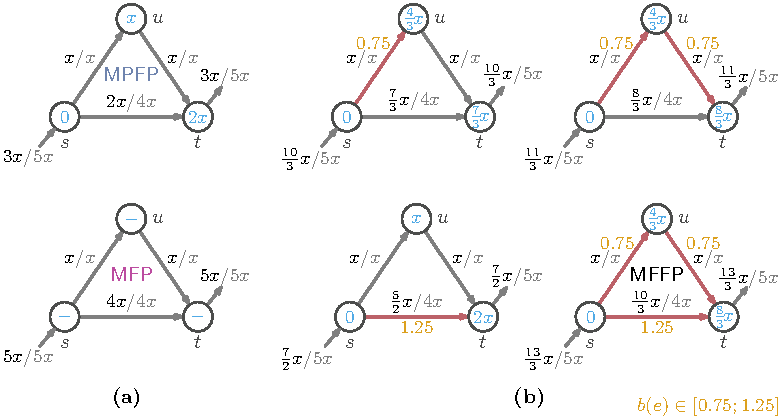
\includegraphics[page=1]{factsplacement/figures/MFF-minimal-example.pdf}
    % 
    \caption[The influence of susceptance scaling.]{A small example graph with
    three vertices, three edges, one source~\source, and one sink~\sink. We
    label each vertex~$\vertexa\in\glssymbol{vertices}$ that is represented by a
    cycle~\tikzVertex with a~\textcolor{THETA}{voltage
    angle~$\glssymbol{voltageangle}(\vertexa)$}. On the edges, we write the
    flow~\glssymbol{flow} and the edge's capacity~\glssymbol{capacity} in the
    form~$\glssymbol{flow} / \textcolor{CAPACITY}{\glssymbol{capacity}}$. Note
    that the \textcolor{SUSCEPTANCE}{susceptance} on the black edges is fixed
    to~$\textcolor{SUSCEPTANCE}{\glssymbol{susceptance}\equiv 1}$ and when
    placing~\textcolor{ColorFACTSedge} {\gls{facts} (red edges)} the
    \textcolor{SUSCEPTANCE}{susceptance} is in the
    range~\textcolor{SUSCEPTANCE}{$\glssymbol{susceptance}(\edge)\in [0.75;
    1.25]$} for all~$\edge\in\glssymbol{factsbranch}$. (a) The top graph shows
    an~$\gls{mpf}(\glssymbol{network})$ with a value
    of~$\opt_{\gls{mpfp}}(\glssymbol{network}) = 3x$. The bottom graph shows
    a~$\gls{mf}(\glssymbol{network})$ with a value of~$\opt_{\gls{mfp}}
    (\glssymbol{network}) = 5x$. (b) Different placement of~\gls{facts} and
    their best \textcolor{SUSCEPTANCE}{susceptance scaling} for this situation
    result in different values for the resulting flow. However, the best
    placement is shown in the bottom right yielding
    a~$\gls{mff}(\glssymbol{network})$ with a value
    of~$\opt_{\gls{mffp}}(\glssymbol{network}) = \nicefrac{13}{3} \cdot x$.}
    % 
    \label{ch:facts:fig:MFF-minimal-example}
\end{figure}
% 
Next, we define the edge costs. It is well known that a convex, piecewise linear
edge cost function~$h$ can easily be modeled in a flow network by replacing the
respective edge~$(\vertexa, \vertexb)$ with as many copies as the linear pieces
of the cost function. The edge capacities are defined by the differences between
consecutive breakpoints of~$h$ and sum up to~$\glssymbol{capacity}(\vertexa,
\vertexb)$; the individual costs correspond to the costs as defined by the
linear pieces between the breakpoints. Thus for ease of presentation we refrain
from explicitly modeling convex piecewise linear cost functions
in~\glssymbol{network}. We rather assume that the flow cost~$z_\lambda$ is given
for each edge~$ (\vertexa,\vertexb)\in\glssymbol{edges}$ with~$\vertexa \ne
\source$ and~$\vertexb \ne
\sink$ by the weighted loss function~$
z_\lambda((\vertexa,\vertexb),\glssymbol{flow})
\coloneqq 
(1-\lambda) 
\cdot 
\ell_{\{\vertexa,\vertexb\}}
(\glssymbol{flow}(\vertexa,\vertexb)) 
% 
$, where $\lambda$ is the weight parameter of~\cref{ch:facts:eq:objective}. The
edges~$(\source,\vertexa)$ from the source~\source to a
generator~$\vertexa\in\glssymbol{generators}$ have
cost~$z_\lambda((\source,\vertexa),\glssymbol{flow}) \coloneqq \lambda \cdot
\fcost{\vertexa}( \glssymbol{flow} ( \source, \vertexa ) )$ and the edges
incident to the sink~\sink have cost~$0$. Then the objective function to be
minimized is~$z_\lambda ( \glssymbol{flow} ) \coloneqq \sum_{\edge \in
\glssymbol{edges}} z_\lambda (
\edge,\glssymbol{flow} )$. Finally, we set the target flow value~$x$ to the total
demand~$\sum_{\vertexa\in \glssymbol{consumers}}
\glssymbol{realpowerdemand}(\vertexa)$ of all consumers. By construction, every
feasible minimum-cost flow in~\glssymbol{network} is a feasible minimum-cost
flow in the underlying power grid~\glssymbol{graph} and vice versa.
% 
%%%%%%%%%%%%%%%%%%%%%%%%%%%%%%%%%%%%%%%%%%%%%%%%%%%%%%%%%%%%%%%%%%%%%%%%%%%%%%%%
\section{Complexity} 
\label{ch:facts:sec:complexity}
%%%%%%%%%%%%%%%%%%%%%%%%%%%%%%%%%%%%%%%%%%%%%%%%%%%%%%%%%%%%%%%%%%%%%%%%%%%%%%%%
%
In the above section we gave no restriction on the control unit's ability. The
latter means that a~\gls{facts} is able to adjust the flow arbitrarily. However,
a realistic~\gls{facts} is only able to adjust the voltage angle difference
within a limited range. Since the proposed hybrid model does not incorporate a
limitation of the power flow scaling, we could instead use the~\gls{dc}-model
and allow to adjust the
susceptances~$\glssymbol{susceptance}(\vertexa,\vertexb)$ arbitrarily, where
either~$\vertexa$ or~$\vertexb$ is in~$\glssymbol{factsbus}$ for~\gls{fcv}s
or~$(\vertexa,\vertexb)\in\glssymbol{factsbranch}$ for~\gls{fce}s. The
limitation for adjusting the voltage angle difference can be modeled by a real
interval~$\interval_{\edge}\in\intervals(\posreals)$ that depends on the
edge~\edge, where~$\intervals (\posreals)$ is the set of all real intervals
and~$\intervals(\posreals)$ is a semiring (\ie, a ring without additive inverse)
of sets. Thus, the interval~$\interval_{\edge}$ is a subset of~\reals that is
defined by the two elements~$x$ and~$y$ with~$x,y\in\interval_{\edge}$
and~$z\in\reals$ such that~$x\leq z\leq y$, which implies
that~$z\in\interval_{\edge}$. The difference now is that either edges incident
to a vertex~\glssymbol{factsbus} for~\gls{fcv}s or all edges
in~$\edge\in\glssymbol{factsbranch}$ for~\gls{fce}s have a variable
susceptance~$%
\glssymbol{susceptance}
\colon
\glssymbol{edges}
\to
\intervals(\posreals)$,
$ 
(\vertexa,\vertexb)
\mapsto
\intervals(\posreals)
$ with~$\vertexa$ or~$\vertexb$ in~\glssymbol{factsbus},
or~$%
\glssymbol{susceptance}
\colon
\glssymbol{factsbranch}
\to
\intervals(\posreals)
% 
$, respectively. An example that shows different scalings for a triangle graph
is given in~\cref{ch:facts:fig:MFF-minimal-example}.
\Cref{ch:facts:fig:MFF-minimal-example} shows different susceptance scaling
of the same graph that lead to different power flows by either allowing more
flow, but fixing the voltage angles, changing the voltage angles and fixing the
flows, or both.

This modeling would change the linear program~\cref{ch:facts:lp:FCV-and-FCE} to
a quadratic program, since~\cref{ch:facts:lp:FCV:eq:electricalfeasible} is a
quadratic constraint with variables~\glssymbol{flow}, \glssymbol{voltageangle},
and~\glssymbol{susceptance}. More precisely, it represents a bilinear
constraint. In~\cref{ch:facts:eq:bilinear} we use a bilinear form,
where~$\bilinearmap\colon\glssymbol{vertices}\times
\glssymbol{vertices}\to\reals$ with~$(\vertexa,\vertexb)\mapsto\glssymbol{susceptance}
(\vertexa,\vertexb) \cdot ( \glssymbol{voltageangle}(\vertexb) - \glssymbol{voltageangle}(\vertexa) )$.
The latter bilinear form is skew-symmetric.
% 
\begin{subequations}
    \begin{align}
    \glssymbol{flow}(\vertexa,\vertexb) 
    &= 
    \glssymbol{susceptance}(\vertexa,\vertexb) 
    (\glssymbol{voltageangle}(\vertexb) 
    - \glssymbol{voltageangle}(\vertexa))
    % 
    \label{ch:facts:eq:bilinear:1}
\\
    \glssymbol{flow}(\vertexa,\vertexb) 
    &= 
    \glssymbol{susceptance}(\vertexa,\vertexb)\cdot\glssymbol{voltageangle}(\vertexb)
    -
    \glssymbol{susceptance}(\vertexa,\vertexb)\cdot\glssymbol{voltageangle}
    (\vertexa)
    % 
    \label{ch:facts:eq:bilinear:2}
% \\
%     \glssymbol{flow}(\vertexa,\vertexb) 
%     &=
%     \bilinearmap(\glssymbol{susceptance}(\vertexa,\vertexb),
%     \glssymbol{voltageangle}(\vertexb))
%     -
%     \bilinearmap(\glssymbol{susceptance}(\vertexa,\vertexb),
%     \glssymbol{voltageangle}(\vertexa))
%     % 
%     \label{ch:facts:eq:bilinear:3}
\\
    \glssymbol{flow}(\vertexa,\vertexb) 
    &=
    \bilinearmap(\glssymbol{susceptance}(\vertexa,\vertexb),
    \glssymbol{voltageangle}(\vertexb)
    - \glssymbol{voltageangle}(\vertexa))
    % 
    \label{ch:facts:eq:bilinear:4}
\end{align}
    \label{ch:facts:eq:bilinear}
\end{subequations}
% 
Thus, we have one quadratic constraint (\ie, the~\gls{kvl} combined with
Ohm's law). However, the other constraints and---in terms of maximizing the
throughput---also the objective stays linear. 
% 
In the first problem, we assume a given placement of the~\gls{facts} and are
just interested in the susceptance scaling, which is~\NP-hard under the
condition that there are quadratic constraints and the objective is linear
[Sahni,1974]. The proof uses a reduction from the~\PartitionP. For more precise
information about the complexity of quadratic programming refer
to~\textcite[p.245; MP2]{Gar79} and~\textcite[p.447; MP5]{Aus99}.
%
% Problem
\begingroup
    %%%%%%%%%%%%%%%%%%%%%%%%%%%%%%%%%%% Problem %%%%%%%%%%%%%%%%%%%%%%%%%%%%%%%%%%%%
\begin{problem}[framed]{\MFFP 
with~\glssymbol{factsbranch}~$\mffp(\glssymbol{network},\glssymbol{factsbranch})$}%
    Instance:  & A network~\glssymbol{network}, and a
    set~$\glssymbol{factsbranch}\subseteq\glssymbol{edges}$.\\
    % 
    Objective: & Find a susceptance
    setting~$\glssymbol{susceptance}\in\interval_{\edge}$ for
    all~$\edge\in\glssymbol{factsbranch}$ such
    that~$\opt_{\gls{mpfp}}(\glssymbol{network})$ is maximum among all choices
    of~\glssymbol{susceptance}.
\end{problem}%
    \label{ch:facts:problem:maximum-facts-flow-problem-with-Ef-optimization-problem}
\endgroup
%
% Note that for the minimum cost flow
% the objective function is piecewise-linear.
% 
%%%%%%%%%%%%%%%%%%%%%%%%%%%%%%%%%%%%%%%%%%%%%%%%%%%%%%%%%%%%%%%%%%%%%%%%%%%%%%%%
\paragraph{Problem Definitions}
\label{ch:facts:sec:complexity:problem-definition}
%%%%%%%%%%%%%%%%%%%%%%%%%%%%%%%%%%%%%%%%%%%%%%%%%%%%%%%%%%%%%%%%%%%%%%%%%%%%%%%%
% 
We can now give different level of granularity for the problem definition of
the~\acrlong{mffp} (\gls{mffp}). Recall
from~\cref{ch:network-analysis} the~\acrlong{mpfp}~$\gls{mpfp}(
\glssymbol{network})$ and its value~$\opt_{\gls{mpfp}}(\glssymbol{network})$.
For simplicity and for consistency reasons, we only consider~\gls{fce}s.
However, all formulations can be translated to~\gls{fcv}s, too. The first
placement problem~$\gls{mffp}(\glssymbol{network},k)$ considers the problem with
a fixed number of~\facts---meaning~$\fmagnitude{\glssymbol{factsbranch}} =
k$---and is defined by~$\opt_{\gls{mffp}}(\glssymbol{network}, k) \coloneqq
\max_{\glssymbol{factsbranch}\subseteq\glssymbol{edges},\glssymbol{susceptance}\in
\interval_{\glssymbol{susceptance}}}\opt_{\gls{mpfp}}(\glssymbol{network})$
with~$\fmagnitude{\glssymbol{factsbranch}} = k$. The optimization problem is
defined as follows.
%
\begingroup
    %%%%%%%%%%%%%%%%%%%%%%%%%%%%%%%%%%% Problem %%%%%%%%%%%%%%%%%%%%%%%%%%%%%%%%%%%%
\begin{problem}[framed]{\MFFP with~$k$-\facts~$\mffp(\glssymbol{network},k)$}%
    % 
    Instance:  & A network~\glssymbol{network}, and parameter~$k\in\naturals$.\\
    % 
    Objective: & Find a set~$\glssymbol{factsbranch}\subseteq\glssymbol{edges}$
    of~\gls{facts} with~$\fmagnitude{\glssymbol{factsbranch}} = k$ and a
    susceptance setting~$\glssymbol{susceptance}\in\interval_{\edge}$ for
    all~$\edge\in\glssymbol{factsbranch}$ such
    that~$\opt_{\gls{mpfp}}(\glssymbol{network})$ is maximum among all choices
    of~\glssymbol{factsbranch} and~\glssymbol{susceptance}.
    % 
    \label{problems:facts:MFF:N-k}
    % 
\end{problem}%
    \label{ch:facts:problems:maximum-facts-flow-with-k-facts-optimization-problem}
\endgroup
% 
Note that if~$\fmagnitude{\glssymbol{factsbranch}} =
\fmagnitude{\glssymbol{edges}} = k$ and the susceptance is defined
in~$\glssymbol{susceptance}(\edge)\in[0,\infty]$ for
all~$\edge\in\glssymbol{factsbranch}$ the value
of~$\opt_{\gls{mffp}}(\glssymbol{network},k) =
\opt_{\gls{mfp}} (\glssymbol{network})$. Assume, we have no limitation on the
number of~\facts we can place. The problem to get the maximum possible flow for
a network~\glssymbol{network} by allowing as many~\gls{facts} as possible (\ie,
some $k$) is called~$\gls{mffp}(\gls{network})$ and its value is denoted
by~$\opt_{
\gls{mffp}}(
\glssymbol{network})\coloneqq\max_{k}
\opt_{\gls{mffp}}(\glssymbol{network},k)$. The problem is defined as follows.
%
\begingroup
    %%%%%%%%%%%%%%%%%%%%%%%%%%%%%%%%%%% Problem %%%%%%%%%%%%%%%%%%%%%%%%%%%%%%%%%%%%
\begin{problem}[framed]{\MFFP~$\mffp(\glssymbol{network})$}%
    % 
    Instance:  & A network~\glssymbol{network}.\\
    % 
    Objective: & Find a set~$\glssymbol{factsbranch}\subseteq\glssymbol{edges}$
    of \gls{facts} with~$\fmagnitude{\glssymbol{factsbranch}} = k$, $0\leq k\leq
    \fmagnitude{\edges}$, and a susceptance
    setting~$\glssymbol{susceptance}\in\interval_{\edge}$ for
    all~$\edge\in\glssymbol{factsbranch}$ such
    that~$\opt_{\mpfp}(\glssymbol{network})$ is maximum among all choices
    of~\glssymbol{factsbranch}, \glssymbol{susceptance}, and~$k$.
    % 
\end{problem}%
    \label{ch:facts:problems:maximum-facts-flow-optimization-problem}
\endgroup
% 
In the simulations, where we allow a susceptance range
of~$\glssymbol{susceptance} (\edge)\in[0,\infty]$, we will see that a small
number of control units suffices to get~$\opt_{\gls{mfp}}(\glssymbol{network})$.
However, dependent on the susceptance interval~$\interval_{\edge}$ and the
network's underlying graph structure,
the~$\opt_{\gls{mffp}}(\glssymbol{network})$ does not necessarily have the same
value as the~$\opt_{\gls{mfp}}(\glssymbol{network})$ meaning~$
\opt_{\gls{mffp}}(\glssymbol{network})
\leq
\opt_{\gls{mfp}}(\glssymbol{network})
$.%

In the simulations, we will be interested in the problem of finding the minimum
number of control units, which we call~$\gls{mnfp}(\glssymbol{network})$. Its
value is denoted by~$
\opt_{\gls{mnfp}}(\glssymbol{network}) 
\coloneqq
\min_{\opt_{\gls{mffp}}(\glssymbol{network},k) 
= 
\opt_{\gls{mffp}}(\glssymbol{network})} k
% 
$.
%
\begingroup
    %%%%%%%%%%%%%%%%%%%%%%%%%%%%%%%%%%% Problem %%%%%%%%%%%%%%%%%%%%%%%%%%%%%%%%%%%%
\begin{problem}[framed]{\MNFP~$\mnfp(\glssymbol{network})$}%
    Instance:  & A network~\glssymbol{network}, and a
    parameter~$k\in\naturals$.\\
    % 
    Objective: & Find a set~$\glssymbol{factsbranch}\subseteq\glssymbol{edges}$
    of~\facts and a susceptance
    setting~$\glssymbol{susceptance}\in\interval_{\edge}$
    with~$\edge\in\glssymbol{factsbranch}$ such that~$k =
    \fmagnitude{\glssymbol{factsbranch}}$ is minimum among all choices
    of~$\opt_{\gls{mffp}}(\glssymbol{network})$.
    % 
    % 
\end{problem}%
    \label{ch:facts:problems:minimum-number-of-facts}
\endgroup
% 
From~\cref{lem:opt_relation_mpf_msf_mf}, we know the bounds of~\gls{mtsfp}. A
similar relationship holds for the~\gls{mffp}, which we describe
in~\cref{lem:opt_relation_mpf_mff_mf}.
% 
%%%%%%%%%%%%%%%%%%%%%%%%%%%%%%%%%%%% LEMMA %%%%%%%%%%%%%%%%%%%%%%%%%%%%%%%%%%%%
\begin{lemma}
    % 
    $\opt_{\gls{mpfp}}(\gls{network})
    \leq
    \opt_{\gls{mffp}}(\gls{network})
    \leq
    \opt_{\gls{mfp}}(\gls{network})$.
    % 
    \label{lem:opt_relation_mpf_mff_mf}
    % 
\end{lemma}
% 
In addition, we can give the following relationship between the aforementioned
problems that is given by the problem definition itself.
%
%%%%%%%%%%%%%%%%%%%%%%%%%%%%%%%%%%%% LEMMA %%%%%%%%%%%%%%%%%%%%%%%%%%%%%%%%%%%%
\begin{lemma}
  $\gls{mpfp}(\glssymbol{network})\subseteq
  % \gls{mff}(\glssymbol{network},\glssymbol{factsbranch})\subseteq
  \gls{mffp}(\glssymbol{network},k)\subseteq
  \gls{mffp}(\glssymbol{network})\subseteq
  \gls{mnfp}(\glssymbol{network})$.
  % 
  \label{lem:problem_relation_mff_mnf}
\end{lemma}
% 
Note that the~\gls{kvl} constraint is a bilinear constraint that can be
reformulated as shown
in~\crefrange{ch:facts:eq:bilinear:1}{ch:facts:eq:bilinear:4}
% 
%%%%%%%%%%%%%%%%%%%%%%%%%%%%%%%%%%%%%%%%%%%%%%%%%%%%%%%%%%%%%%%%%%%%%%%%%%%%%%%%
\paragraph{Overview}
\label{ch:facts:sec:complexity:overview}
%%%%%%%%%%%%%%%%%%%%%%%%%%%%%%%%%%%%%%%%%%%%%%%%%%%%%%%%%%%%%%%%%%%%%%%%%%%%%%%%
%
For trees
(see~\cref{ch:switching:sec:complexity:tbl:complexity-overview}--\screen{1}) any
of the aforementioned problems is polynomial time solvable, since we
reach~$\opt_{\gls{mfp}}(\gls{network})$ without any control units. We will
discuss this in more detail in~\cref{ch:facts:sub:hybridtheory}. While
increasing the structural complexity of a graph by allowing cycles,
\textcite[pp.10ff.; Theorem 4]{Leh15a} show that the problem is already~\NP-hard
for cacti with maximum degree of~$3$ by reduction from~\SSP (\ssp;
see~\cref{ch:switching:sec:complexity:subsec:np_hardness_Source_Sink_MTSF_capacity1}).
In~\cref{ch:switching:sec:complexity:tbl:complexity-overview}--\screen{3}, we
give a short overview. For the most general graph structure---meaning an
arbitrary graph---the problem is strongly~\NP-hard. The latter was shown
by~\textcite[pp. 7; Theorem 1]{Leh15a} by reduction from~\emph{exact cover by
3-set problem} (\ie, given a set~$U$ and a set of subsets~$M\subseteq
\mathcal{P}(U)$ with~$\fmagnitude{M}=3$ the decision problem is whether there is
a set~$M'\subseteq M$ such that~$\bigcup\{X\mid X\in M'\} = U$) and an overview
on that is given
in~\cref{ch:switching:sec:complexity:tbl:complexity-overview}--\screen{5}. Note
that~\textcite{Leh15a} implemented this by a choice network and focused on the
problem~$\mffp(\glssymbol{network},\glssymbol{factsbranch})$, where the position
of the~\gls{facts} is predefined.
%
%%%%%%%%%%%%%%%%%%%%%%%%%%%%%%%%%%%%%%%%%%%%%%%%%%%%%%%%%%%%%%%%%%%%%%%%%%%%%%%
\begin{landscape}
    \begin{table}
        % 
        % latex table generated in R 3.2.2 by xtable 1.8-0 package
% Wed Jan 27 11:17:04 2016
{\setlength{\tabcolsep}{0.3em}}
{\renewcommand{\arraystretch}{1}}% for the vertical padding
% \small
\begin{tabular}{%
  l>{\centering\arraybackslash}%
  m{1.5cm}>{\centering\arraybackslash}%
  m{3.0cm}>{\centering\arraybackslash}%
  m{1.7cm}cccc>{\centering\arraybackslash}%
  m{2.7cm}>{\centering\arraybackslash}%
  m{2.7cm}>{\centering\arraybackslash}%
  m{1.1cm}cc%
}%
\toprule
  & \multirow[c]{2}*{\textbf{Problem}}
  & \multicolumn{6}{c}{\textbf{Network Properties}}
  & \multicolumn{2}{c}{\textbf{Complexity} }
  & \multicolumn{3}{c}{\textbf{Algorithms}}
  \\
%-------------------------------------------------------------------------------
%-------------------------------------------------------------------------------
 \cmidrule(lr){3-8}\cmidrule(lr){9-10}\cmidrule(lr){11-13}
  &
  & \multicolumn{1}{c}{Graph Structure}
  & \multicolumn{1}{c}{Example}
  & \screentextcolor{GENERATOR}{$\fmagnitude{\generators}$} 
  & \screentextcolor{CONSUMER}{$\fmagnitude{\consumers}$}
  & \screentextcolor{SUSCEPTANCE}{$\susceptance$}
  & \screentextcolor{CAPACITY}{$\capacity$}
  & \multicolumn{1}{c}{Hardness}
  & \multicolumn{1}{c}{Reference}
  & \multicolumn{1}{c}{Name} 
  & \multicolumn{1}{c}{\screentextcolor{SUSCEPTANCE}{$\susceptance$}}
  & \multicolumn{1}{c}{\screentextcolor{CAPACITY}{$\capacity$}}
  \\
%-------------------------------------------------------------------------------
%-------------------------------------------------------------------------------
 \midrule\addlinespace
%-------------------------------------------------------------------------------
%-------------------------------------------------------------------------------
\rowcolor{Table-Line-Marker}
%-------------------------------------------------------------------------------
1\label{ch:facts:sec:exploit_structural_characteristics:tbl:tree}
& \acrshort{mffp} and~\acrshort{offp}
& tree graphs
& \raisebox{-0.5cm}[0pt][0pt]{
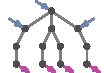
\includegraphics{switchplacement/figures/graph_structure-tree.pdf}%
}
& \screentextcolor{GENERATOR}{$\infty$}
& \screentextcolor{CONSUMER}{$\infty$}
& \screentextcolor{SUSCEPTANCE}{--}
& \screentextcolor{CAPACITY}{--}
& polynomial-time solvable
& \cref{ch:network-analyzes:sec:mathematical-model:lem:pf-matrix-is-tum},
\cref{ch:facts:thm:fvs}, 
\cref{ch:foundations:sec:graph-theoretical-flows} p.\
\pageref{ch:foundations:sec:graph-theoretical-flows:para:maximum-flow-problem}
& \acrshort{mf}
& \screentextcolor{SUSCEPTANCE}{$\infty$}
& \screentextcolor{CAPACITY}{$\infty$}
\\\addlinespace\addlinespace
% 
2\label{ch:switching:sec:exploit_structural_characteristics:tbl:series_parallel}
& \acrshort{mffp} and~\acrshort{offp}
& series-parallel graphs
& 
\raisebox{-0.5cm}[0pt][0pt]{%
  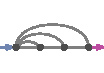
\includegraphics{switchplacement/figures/graph_structure-series_parallel_graph.pdf}%
}%
& \screentextcolor{GENERATOR}{$\infty$}
& \screentextcolor{CONSUMER}{$\infty$}
& \screentextcolor{SUSCEPTANCE}{$\infty$}
& \screentextcolor{CAPACITY}{$\infty$}
& --%\NP-hard
& --%\parencite[pp. 10; Theorem 4]{Leh15a}
& --
& \screentextcolor{SUSCEPTANCE}{--}
& \screentextcolor{CAPACITY}{--}
\\\addlinespace\addlinespace
% 
\rowcolor{Table-Line-Marker}
%-------------------------------------------------------------------------------
3\label{ch:facts:sec:exploit_structural_characteristics:tbl:cactus}
& \acrshort{mffp} and~\acrshort{offp}
& cacti with maximum degree of~$3$
& \raisebox{-0.5cm}[0pt][0pt]{%{-\totalheight}
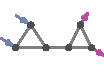
\includegraphics{switchplacement/figures/graph_structure-cacti_graph.pdf}}
& \screentextcolor{GENERATOR}{$\infty$}
& \screentextcolor{CONSUMER}{$\infty$}
& \screentextcolor{SUSCEPTANCE}{$\infty$}
& \screentextcolor{CAPACITY}{$\infty$}
& \NP-hard
& \parencite[pp.10; Theorem 4]{Leh15a}
& --
& \screentextcolor{SUSCEPTANCE}{--}
& \screentextcolor{CAPACITY}{--}
\\\addlinespace\addlinespace
% 
4\label{ch:switching:sec:exploit_structural_characteristics:tbl:plane_graph}
& \acrshort{mffp} and~\acrshort{offp}
& planar graph with~$\max$ degree of~$3$
& \raisebox{-0.5cm}[0pt][0pt]{%
  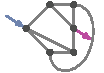
\includegraphics{switchplacement/figures/graph_structure-plane_graph.pdf}
}%
& \screentextcolor{GENERATOR}{$\infty$}
& \screentextcolor{CONSUMER}{$\infty$}
& \screentextcolor{SUSCEPTANCE}{$\infty$}
& \screentextcolor{CAPACITY}{$\infty$}
& --
& --
& --
& \screentextcolor{SUSCEPTANCE}{--}
& \screentextcolor{CAPACITY}{--}
\\\addlinespace\addlinespace
% 
\rowcolor{Table-Line-Marker}
%-------------------------------------------------------------------------------
5
\label{ch:facts:sec:exploit_structural_characteristics:tbl:arbitrary_graph}
& \acrshort{mffp} and~\acrshort{offp}
& arbitrary graphs
& \raisebox{-0.5cm}[0pt][0pt]{%{-\totalheight}

\includegraphics{switchplacement/figures/graph_structure-arbitrary_graph.pdf}%
}%
& \screentextcolor{GENERATOR}{$\infty$}
& \screentextcolor{CONSUMER}{$\infty$}
& \screentextcolor{SUSCEPTANCE}{$\infty$}
& \screentextcolor{CAPACITY}{$\infty$}
& strongly~\NP-hard
& \parencite[pp.7; Theorem 1]{Leh15a}
& --
& \screentextcolor{SUSCEPTANCE}{--}
& \screentextcolor{CAPACITY}{--}
\\\addlinespace\addlinespace
% 
%-------------------------------------------------------------------------------
%-------------------------------------------------------------------------------
   \bottomrule
\end{tabular}

        % 
        \caption[Overview of results on the complexity of FACTS
        placement.] {Overview of known results on the complexity of
        the~\gls{mff} and~\gls{off} problem. The complexity increases
        from top to bottom as shown in the hardness column. Note that the main
        points that influence the complexity of the problem are the graph
        structure of~\glssymbol{graph}, the number of \screentextcolor{GENERATOR}
        {generators~$\glssymbol{generators}$}, the number of \screentextcolor{CONSUMER}
        {consumers~$\glssymbol{consumers}$}, the
        \screentextcolor{SUSCEPTANCE}{susceptance~\glssymbol{susceptance}}, and the
        \screentextcolor{CAPACITY}{capacity~$\glssymbol{capacity}$}. 
        % If there are multiple
        % results or if the results differ for~\gls{mtsf} and~\gls{ots},
        % we colored the relating entries in~\myhl{KITpalegreen15}{green}.
        }%
        % 
        \label{ch:switching:sec:complexity:tbl:complexity-overview}
        % 
    \end{table}
\end{landscape}
%
% %%%%%%%%%%%%%%%%%%%%%%%%%%%%%%%%%%%%%%%%%%%%%%%%%%%%%%%%%%%%%%%%%%%%%%%%%%%%%%%%
% \paragraph{NP-hardness of Source-Sink-MFF on Series-Parallel-Graphs}
% \label{ch:facts:sec:complexity:overview}
% %%%%%%%%%%%%%%%%%%%%%%%%%%%%%%%%%%%%%%%%%%%%%%%%%%%%%%%%%%%%%%%%%%%%%%%%%%%%%%%%
% %
% For the $\mff(\glssymbol{network}, \glssymbol{factsbranch})$, we can simply adapt the proof
% in~\cref{ch:switching:sec:complexity:subsec:np_hardness_Source_Sink_MTSF_capacity1}
% by allowing a susceptance range from~$[0,x]$ on the~$(\vertex_i,\vertex_{i+1})$
% edges, where~$x$ is the original susceptance~\glssymbol{susceptance}. Then~$0$ would
% basically present a switching on that particular edge. Note that the total
% susceptance of the path over~$\vertexa_i$ is given
% by~$$\glssymbol{susceptance}(\apath(\vertex_i, \vertexa, \vertex_{i+1})) 
% = \frac{1}{\frac{1}{\frac{2}{k+w_i}} 
% + \frac{1}{\frac{2}{k + w_i}}} = \frac{1}{k + w_i}.$$ The susceptance of an
%   edge~$(\vertex_i,\vertex_{i+1})$ is within the
%   interval~$\interval_{\edge}\in[0,\nicefrac{1}{k}-\nicefrac{1} {k+w_i}]$.
% % 
% Since the~$\lim_{\glssymbol{susceptance}(\vertex_{i},\vertex_{i+1})\rightarrow 0}\frac{1}
% {k+w_i} + \frac{1}{k} - \frac{1}{k+w_i} = \frac{1}{k+w_i}$ the voltage angle
% difference is given by~$\lim_{\glssymbol{susceptance}(\vertex_{i},\vertex_{i+1})\rightarrow
% 0}\deltaangle(\vertex_i, \vertex_{i+1}) = k + w_i$. Note that the
% susceptance~$\glssymbol{susceptance}(\source, \sink)$ is fixed to~$\nicefrac{1}{1+(n+1)k}$
% and the total voltage angle difference is~$\deltaangle(\source, \sink) = 1 + (n
% + 1) k$. Thus, 
% 
% 
\begin{figure}[t!]
    % 
    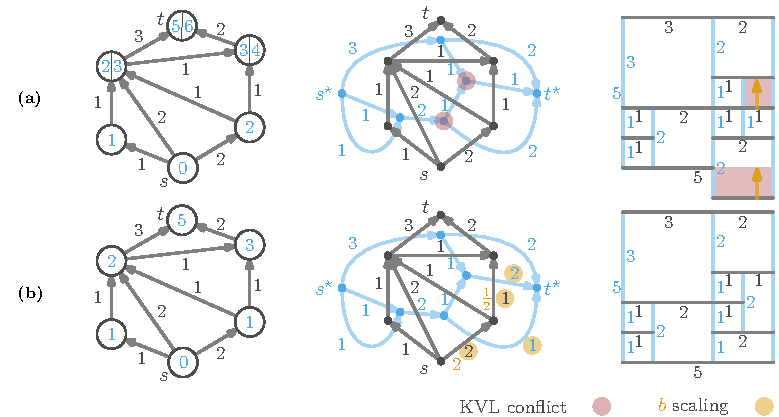
\includegraphics[page=1]{factsplacement/figures/geometric-shifting-example.pdf}
    % 
    \caption[Different interpretations for the~\gls{kvl} conflict and
    resolution.]{The graph
    from~\cref{ch:facts:analogies-susceptance-scaling}~\parencite[p.18; Figure
    18]{Fel13}, where we split the~\textcolor{KVLCONFLICT}{\gls{kvl} conflict}
    step (a) that is a~\gls{kcl} conflict in the \textcolor{DUALGRAPH}{dual
    graph~\glssymbol{dualgraph}} from the susceptance scaling step (b). If not
    described otherwise, we have unit
    susceptances~\textcolor{SUSCEPTANCE}{\glssymbol{susceptance}}
    with~$\textcolor{SUSCEPTANCE}{\glssymbol{susceptance} \equiv 1}$. In (a)
    the~\textcolor{KVLCONFLICT}{\gls{kvl} conflict} is visible in all three
    representations. Whether it is the left graph that shows the conflict by
    non-unique~\textcolor{THETA}{voltage angle~\glssymbol{voltageangle}}
    assignments, or in the middle representation with
    the~\textcolor{KVLCONFLICT}{\gls{kcl} conflicts} in the
    \textcolor{DUALGRAPH}{dual graph~\glssymbol{dualgraph}}, or the
    \textcolor{KVLCONFLICT}{rectangle conflicts} in the geometric representation
    on the right side. However, the susceptance scalings shown in (b) and
    indicated with the~\textcolor{KITorange}{arrows~$\uparrow$} for the
    geometric interpretation in the right most figure in~(a) fix these conflicts
    in all three representations.}
    % 
    \label{ch:facts:fig:geometric-shifting-example}
    % 
\end{figure}
%   
%%%%%%%%%%%%%%%%%%%%%%%%%%%%%%%%%%%%%%%%%%%%%%%%%%%%%%%%%%%%%%%%%%%%%%%%%%%%%%%%
\section{Planar Problem Reinterpretation}
\label{ch:facts:sec:planar}
%%%%%%%%%%%%%%%%%%%%%%%%%%%%%%%%%%%%%%%%%%%%%%%%%%%%%%%%%%%%%%%%%%%%%%%%%%%%%%%%
% 
Recall from~\cref{ch:switching:sec:network_modeling} that we defined a single
source and single sink planar power flow in terms of simultaneous flows in the
primal graph~\glssymbol{graph} and dual graph~\glssymbol{dualgraph}. The
definition of simultaneous flows is given
in~\cref{ch:network-analyzes:simultaneous-flow-representation}. We adjust the
problem formulation for~\gls{facts} in the following, while allowing a
susceptance range of~$[0,\infty]$ for all edges~$\edge\in\glssymbol{edges}$.
% 
\begingroup
    %%%%%%%%%%%%%%%%%%%%%%%%%%%%%%%%%%% Problem %%%%%%%%%%%%%%%%%%%%%%%%%%%%%%%%%%%%
\begin{problem}[framed]{\source-\sink-\gls{dc}~\acrlong{feas} with
\gls{facts}~\source-\sink-\gls{dc}-\gls{feas}-\gls{facts}$(\glssymbol{graph},
\glssymbol{dualgraph},\oneToOneMap)$}%
  Instance: & A plane~\source-\sink-graph~$\glssymbol{graph}$ and its
  dual~$\glssymbol{dualgraph}$,
  subsets~$\glssymbol{edges}_1\subseteq\glssymbol{edges}(\glssymbol{graph})$
  and~$\glssymbol{edges}_2\subseteq\glssymbol{edges} (\glssymbol{dualgraph})$,
  and a bijection~$\oneToOneMap\colon
  \glssymbol{edges}_1 \to \glssymbol{edges}_2$.\\
  % 
  Objective: & Find~\gls{kcl}-feasible flows~$\glssymbol{flow}_{\glssymbol{graph}}$
  and~$\glssymbol{flow}_{\glssymbol{dualgraph}}$ in~$\glssymbol{graph}$
  and~$\glssymbol{dualgraph}$
  with~$\glssymbol{flowvalue}(\glssymbol{graph})\not=0$ and~$
  \glssymbol{flowvalue}(\glssymbol{dualgraph})\not=0$ such that
  for every edge~$\edge\in\glssymbol{edges}$ we
  have~$\glssymbol{flow}_{\glssymbol{graph}}(\edge) =
  \glssymbol{flow}_{\glssymbol{dualgraph}}(\oneToOneMap(\edge))$.
  % 
  % 
\end{problem}%
%%%%%%%%%%%%%%%%%%%%%%%%%%%%%%%%%%%%%%%%%%%%%%%%%%%%%%%%%%%%%%%%%%%%%%%%%%%%%%%%
    \label{ch:facts:problems:facts-simultaneous-flow-problem}
\endgroup
%
Instead of demanding that the bijection of the flows holds for all edges, we
relax this property to edges
in~$\glssymbol{edges}\setminus\glssymbol{factsbranch}$.
In~\cref{ch:facts:fig:geometric-shifting-example}, we apply a feasible
flow~\glssymbol{flow} on the primal graph~\glssymbol{graph} and show that an
adjustment of the susceptances transforms~\glssymbol{flow} into a feasible power
flow. However, the assumption to~$[0,\infty]$ is quite strong. Thus, restricting
the height scaling would lead to the same formulation as
in~\cref{ch:network-analysis}.
%
%%%%%%%%%%%%%%%%%%%%%%%%%%%%%%%%%%%%%%%%%%%%%%%%%%%%%%%%%%%%%%%%%%%%%%%%%%%%%%%%
\section{Placing Flow Control Buses} 
\label{ch:facts:sec:hybridmodel}
%%%%%%%%%%%%%%%%%%%%%%%%%%%%%%%%%%%%%%%%%%%%%%%%%%%%%%%%%%%%%%%%%%%%%%%%%%%%%%%%
% 
In this section we seek to answer the question of how many flow control buses are
necessary to obtain a globally optimal solution. Recall that the flow model is a
relaxation of the physical model and uses fewer constraints. Therefore, optimal
solutions in the flow model are at least as good as in the physical model.

Given a power grid~$\glssymbol{graph} = ( \glssymbol{vertices},
\glssymbol{edges} )$, we say that making the vertices in~\glssymbol{factsbus}
flow control vertices achieves~\emph{full control} if the objective value of an
optimal energy flow for the grid~$\glssymbol{graph}_{\glssymbol{factsbus}}$ is
the same as the objective value of an optimal solution in the flow model (or
equivalently in the hybrid network~$\glssymbol{graph}_{\glssymbol{vertices}}$,
where every vertex is a flow control vertex). Our experiments indicate that in
the~\gls{ieee} instances a small fraction of the vertices is often sufficient to
achieve full control as was already indicated
in~\cref{ch:facts:analogies-susceptance-scaling}. Afterwards we give a
graph-theoretical explanation of this behavior.
%
%%%%%%%%%%%%%%%%%%%%%%%%%%%%%%%%%%%%%%%%%%%%%%%%%%%%%%%%%%%%%%%%%%%%%%%%%%%%%%%%
\subsection{Experiments}
\label{ch:facts:sub:experiments-control-units}
%%%%%%%%%%%%%%%%%%%%%%%%%%%%%%%%%%%%%%%%%%%%%%%%%%%%%%%%%%%%%%%%%%%%%%%%%%%%%%%%
% 
%
\begin{table}[tb!]
    \centering\small
    % 
    \begin{tabular}{lrrrr}
        \toprule
        \multicolumn{1}{c}{case} & \multicolumn{1}{c}{$\fmagnitude{\glssymbol{vertices}}$}
        & \multicolumn{1}{c}{$\fmagnitude{\glssymbol{edges}}$} &
        \multicolumn{1}{c}{$\fmagnitude{\glssymbol{generators}}$} &
        \multicolumn{1}{c}{$\glssymbol{realpowerdemand}$} \\
        \midrule
        \texttt{case6} &   6 &  11 &   3 & 210.00 \\ 
        \texttt{case9} &   9 &   9 &   3 & 315.00 \\ 
        \texttt{case14} &  14 &  20 &   5 & 259.00 \\ 
        \texttt{case30} &  30 &  41 &   6 & 189.20 \\ 
        \texttt{case39} &  39 &  46 &  10 & 6254.23 \\ 
        \texttt{case57} &  57 &  78 &   7 & 1250.80 \\ 
        \texttt{case118} & 118 & 179 &  54 & 4242.00 \\ 
        \bottomrule
    \end{tabular}
    % 
    \caption[\gls{ieee} Benchmark Set Structure.]{\gls{ieee} benchmark
    set with~$\fmagnitude{\glssymbol{vertices}}$, $\fmagnitude{\glssymbol{edges}}$,
    $\fmagnitude{\glssymbol{generators}}$, and $\glssymbol{realpowerdemand}$ representing number of
    buses, number of transmission lines, number of generators and total power
    demand, respectively.}
    \label{ch:facts:tab:examples}
\end{table}
%
For our evaluation we use the~\gls{ieee} benchmark data sets
\parencite{online:IEEEtestData,Zimmerman2011} shown
in~\cref{ch:facts:tab:examples}. There each case is named according to the
number of buses~$\fmagnitude{\glssymbol{vertices}}$.  The number of generators
and the number of edges are denoted by~$\fmagnitude{\glssymbol{generators}}$
and~$\fmagnitude{\glssymbol{edges}}$, respectively.

To obtain piecewise linear functions for generator costs~$\fcost{\vertexa}$ for
all~$\vertexa\in\glssymbol{generators}$ and line losses~$\floss{\edge}$ for
all~$\edge\in\glssymbol{edges}$, we simply sample the cost functions using a specified
number of sampling points. Note further that our approach requires convex cost
functions, but this is fine in practice~\parencite{wood1996power}; in particular
the functions are convex for the~\gls{ieee} benchmark instances.

% >cat /proc/cpuinfo
We performed our experiments on an AMD Opteron 6172 processor running openSUSE
12.2. Our implementation is written in Python 2.7.3 and uses
PYPOWER~\parencite{online:pypower}, a Python port of
MATPOWER~\parencite{Zimmerman2009,Zimmerman2011a}, for computing solutions for
the~\gls{opfp}. For computing solutions and minimizing the number of control
buses in our hybrid model we use the (integer) linear programming solver Gurobi
6.0.0~\parencite{online:Gurobi}.
% 
\begin{figure}[t!]%
    \centering
    \begin{subfigure}[t]{.492\textwidth}
     \centering
         \includegraphics[width=\plotscale\linewidth, page=4,trim=0cm 0cm 0cm
         0cm]{factsplacement/plots/plotCostsVsLosses.pdf}
     \caption{Total costs~\gencost and losses~\losscost for the~\gls{ieee}
     benchmark data with 30 buses, where the square cross marks the solution
     computed by~\gls{opf}.}
     \label{ch:facts:sub:experiments-control-units:fig:plot-costs-losses}
    \end{subfigure}
    %
    \hfill
    \begin{subfigure}[t]{.492\textwidth}
     \centering
         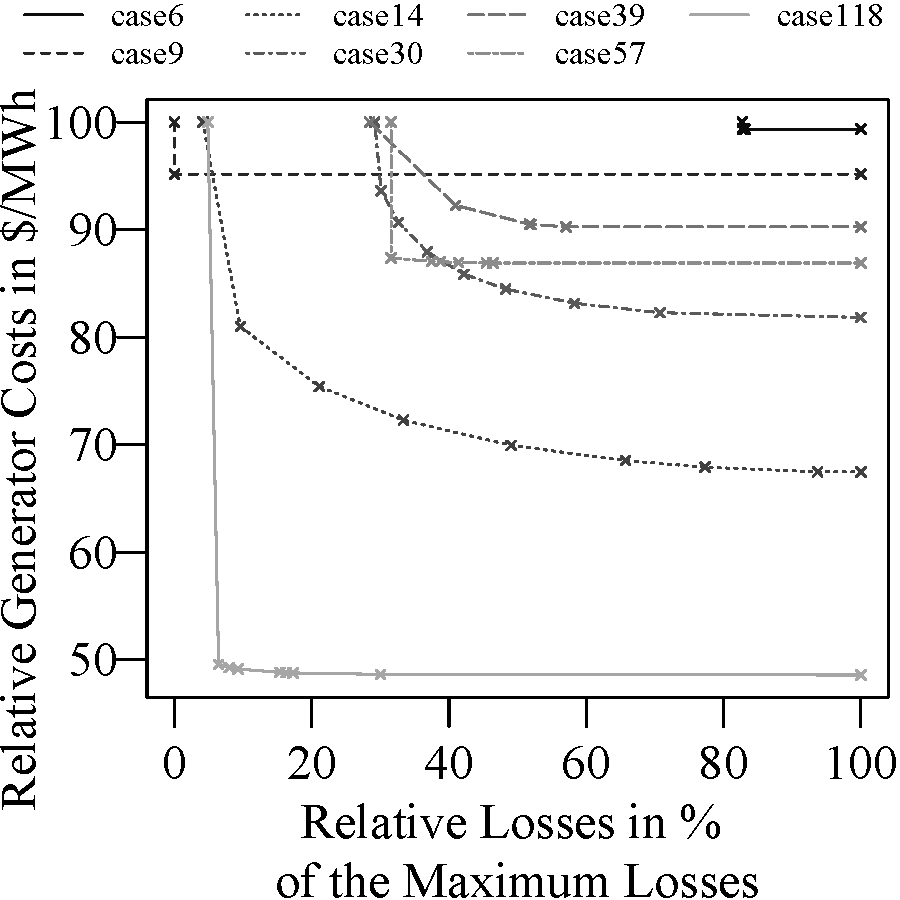
\includegraphics[width=\plotscale\linewidth, page=1,trim=0cm 0cm 0cm 0cm]{factsplacement/plots/plotCostsVsLossesNormalized.pdf}
     \caption{Relative costs and losses for the~\gls{ieee} benchmark data
     sets.}
     \label{ch:facts:fig:plot-costs-losses-normalized}
    \end{subfigure}
    %
    \caption[Trade-off of generator costs~\gencost and losses~\losscost]{Trade-off
        of generator costs~\gencost and losses~\losscost normalized to the
        maximum generator cost ($\lambda = 0$) and the maximum loss ($\lambda =
        1)$ as~$\lambda$ varies from~$0$ to~$1$.}
\end{figure}

First, we observe that the value of~$\lambda$, which controls the weighting of
costs and losses in the objective value, has a significant effect on the
objective values of generator costs and line losses.
\Cref{ch:facts:sub:experiments-control-units:fig:plot-costs-losses} shows the
trade-off for the~\gls{ieee} instance \texttt{case30} (the plots for the
other instances can be found in~\cref{ch:appendix:sec:facts:simulations}).
The~\gls{opf} solution, which ignores losses, is typically at the far end
of the spectrum with high losses and is comparable to our solution
with~$\lambda = 1$.  As can be seen
in~\cref{ch:facts:fig:plot-costs-losses-normalized}, where the costs and losses
are normalized to the maximum cost and the maximum loss per instance, the same
trade-off behavior is present in all instances.  It thus makes sense to allow
the operator of a power grid to choose the value of~$\lambda$ in order to model
the true operation costs.

On the other hand, it may then be the case that the number of flow control
vertices to achieve full control of the network varies depending on the choice
of~$\lambda$. \Cref{ch:facts:fig:plot-controller-weight} shows for different
values of~$\lambda$ the relative number of control vertices necessary to achieve
full control in each of the instances. In most cases less than 15\% of all
vertices need to be controllers to achieve full control.  For the cases with 6
vertices and 14 vertices this percentage is slightly bigger, which is mainly an
artifact stemming from the small total size.  As can be seen, the required
number of units is relatively stable but drops to zero for~$\lambda = 1$, \ie,
when only the generator costs are considered. This is due to the fact that
all~\gls{ieee} instances have basically unlimited line capacities and thus
do not restrict the possible flows.

\begin{figure}[tb!]%
    \centering
    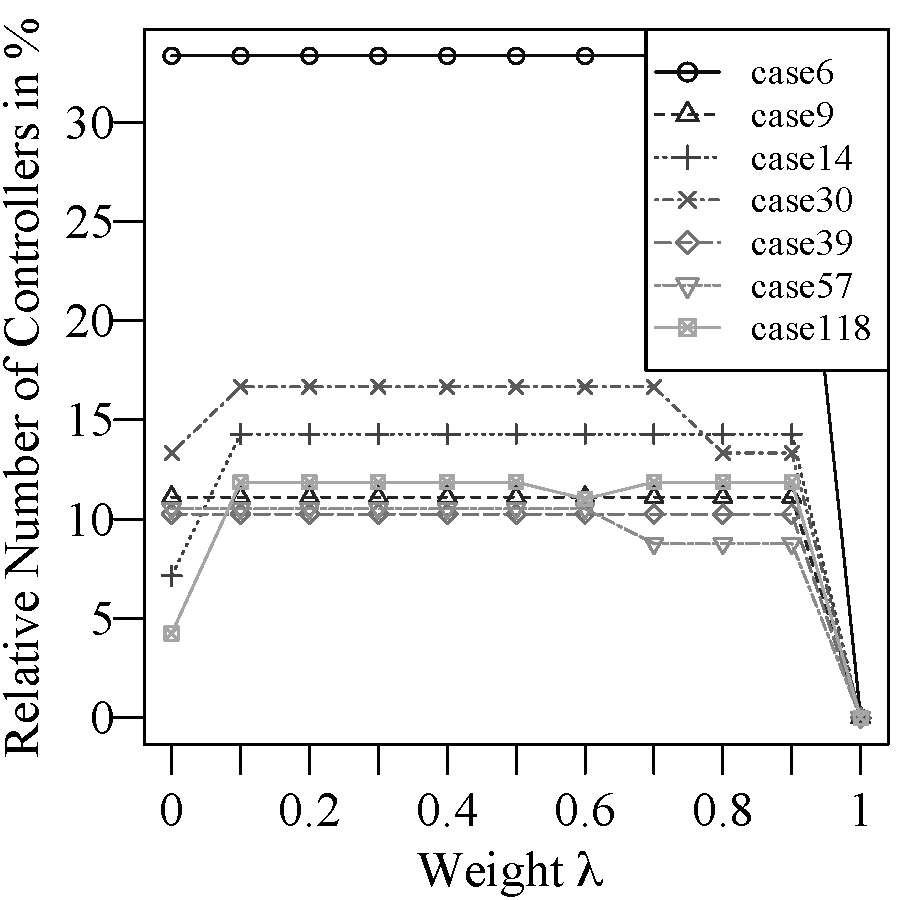
\includegraphics[width=\plotscaleOne\linewidth, trim=0cm 0cm 0cm 0cm]{factsplacement/plots/plotControllerVsWeight.pdf}
    \caption[Comparison of the relative number of controller.]{Relative number
    of controllers for achieving full control in the~\gls{ieee} instances
    as~$\lambda$ varies from~$0$ to~$1$.}%
    \label{ch:facts:fig:plot-controller-weight}%
\end{figure}%

In order to make a useful prediction on the number of vertices required for full
control that applies to all choices of~$\lambda$, in the following we take for
each instance the maximum of the smallest possible number of vertices to achieve
full control over all values of~$\lambda$ and refer to this as the number of
vertices for achieving full control of the instance.  This conservative choice
ensures that the numbers we compute are certainly an upper bound for achieving
full control, independent of the actual choice of~$\lambda$.
%
%%%%%%%%%%%%%%%%%%%%%%%%%%%%%%%%%%%%%%%%%%%%%%%%%%%%%%%%%%%%%%%%%%%%%%%%%%%%%%%%
\subsection{Structure of Optimal Solutions}
\label{ch:facts:sub:hybridtheory}
%%%%%%%%%%%%%%%%%%%%%%%%%%%%%%%%%%%%%%%%%%%%%%%%%%%%%%%%%%%%%%%%%%%%%%%%%%%%%%%%
%
As we have seen in our experimental evaluation, often a small number of flow
control vertices is sufficient to ensure that solutions in the hybrid model are
the same as in the flow model.  In the following we provide a theoretical
explanation of this property and link it to structural properties of power
grids. \textcite{6507352} give similar structural results on spanning trees, but
using a different model.

A first observation is that flow control vertices influence all incident edges.
Thus, if every edge is incident to a flow control vertex, \ie, the
set~$\glssymbol{factsbus}^c$ is a~\emph{vertex cover} of~\glssymbol{graph} (\ie,
$c = 1$), no edge in the network is affected by the
constraint~\cref{ch:facts:eq:electricalflowintro}). Then the flow model and the
hybrid model are equivalent and full control is achieved. However, it is
generally not true that power grids admit small vertex covers; as shown
in~\cref{ch:facts:fig:barchart-cases-controller}, all instances require more
than 40\% of their vertices for a vertex cover. In the following, we show a much
stronger result, namely that it suffices for becoming independent
of~\cref{ch:facts:eq:electricalflowintro} that the native power
grid~$\glssymbol{graph}-{\glssymbol{factsbus}^c}$ is an acyclic network (\ie, $c
= 2$).  Moreover, if~$\lambda = 1$, (line losses are neglected) and edge
capacities are ignored, it even suffices
that~$\glssymbol{graph}-{\glssymbol{factsbus}^c}$ is a so-called \emph{cactus}
graph, in which every edge is part of at most one cycle (\ie, $c = 3$).
%
\begin{figure}[t!]
    \centering
%       trim = left, bottom, right, top
    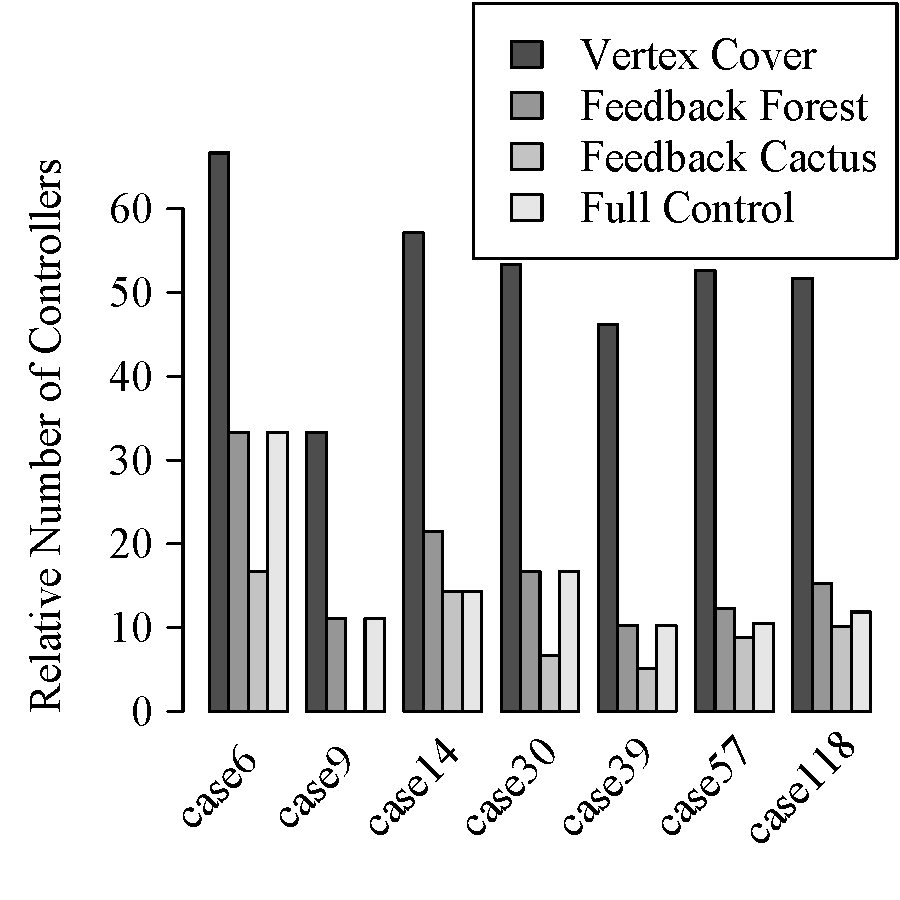
\includegraphics[width=\plotscaleOne\linewidth, trim = 0cm 0cm 0cm 0cm]{factsplacement/plots/plotBarchartCasesVsController.pdf}
    \caption[Comparison of the size of different~$c$-pumpkin hitting sets.]
    {Comparison of the number of vertices which need to be removed from
    the network to get a tree (\ie, $2$-pumpkin hitting set) or a cactus (\ie,
    $3$-pumpkin hitting set), with the worst number of controllers to have full
    control in the network (\ie, equivalent costs to the graph-theoretical
    flow).}
      % 
    \label{ch:facts:fig:barchart-cases-controller}
\end{figure}
%
\begin{lemma} 
    Let~$\subgraph = (\glssymbol{vertices}, \glssymbol{edges})$ be a native
    power grid and let~\vertex be a vertex whose removal disconnects~\subgraph
    into connected components with vertex sets~$\connectedComponent_1, \dots,
    \connectedComponent_k$. Then a flow~\glssymbol{flow} is a feasible
    electrical flow for~\subgraph if and only if it is a feasible electrical
    flow for~$\subgraph_i =
    \subgraph [ \connectedComponent_i \cup \{ \vertex \}]$ for~$i = 1, \dots, k$.
    % 
    \label{ch:facts:lem:decompose-powergrid-cutvertex}
\end{lemma}
%
\begin{proof}
    Clearly, if~$\glssymbol{voltageangle}(\vertexa)$ is a feasible voltage angle assignment
    for all~$\vertexa\in\glssymbol{vertices}(\subgraph)$,
    then its restriction to~$\connectedComponent_i \cup \{ \vertex \}$ is a
    feasible angle assignment for~$\subgraph_i$. Conversely, assume
    that~$\glssymbol{voltageangle}_i$ is a feasible angle assignment for~$\subgraph_i$.
    Define~${\glssymbol{voltageangle}_i}' = \glssymbol{voltageangle}_i -
    \glssymbol{voltageangle}_i (\vertex)$. Since for every edge in~$\subgraph_i$
    the voltage angles of the endpoints are changed by the same value,
    ${\glssymbol{voltageangle}}'$ is a feasible voltage angle assignment
    for~$\subgraph_i$. Further, ${\glssymbol{voltageangle}_i}'(\vertex) = 0$ for
    every~$\subgraph_i$, which means that the function~$\glssymbol{voltageangle}
    \colon
    \glssymbol{vertices}\to \reals$, where~$\glssymbol{voltageangle}(\vertexa)\mapsto
    {\glssymbol{voltageangle}_i}'(\vertexa)$ for~$\vertexa \in
    \connectedComponent_i$ is well-defined. Note that the restriction
    of~\glssymbol{voltageangle} to any of the~$\subgraph_i$ coincides
    with~${\glssymbol{voltageangle}_i}'$.  Since every edge of~\subgraph belongs
    to exactly one of the~$\subgraph_i$, it follows
    that~\glssymbol{voltageangle} is a feasible voltage angle assignment
    for~\subgraph.
\end{proof}
%
Iteratively applying~\cref{ch:facts:lem:decompose-powergrid-cutvertex}
yields the following.
%
\begin{corollary}
    A flow in a native power grid is electrically feasible if and only if it is
    electrically feasible for each biconnected component of the power grid.
    % 
    \label{ch:facts:cor:electrical-feasible-blocks}
\end{corollary}

We observe that if~$\glssymbol{graph} - \glssymbol{factsbus}^c$ is a forest
(\ie, $c = 2$), then each biconnected component~\subgraph consists of a single
edge~$\{ \vertexa, \vertexb
\}$. Then~$\glssymbol{voltageangle} (\vertexa) =
\nicefrac{\glssymbol{flow}(\vertexa,\vertexb)}{
\glssymbol{susceptance}(\vertexa,\vertexb)}$ and~$\glssymbol{voltageangle}
(\vertexb) = 0$ are feasible voltage angles for any flow~\glssymbol{flow}
in~$\glssymbol{graph} -
\ffactsbus{2}$. Thus, we conclude with the following theorem.
%
\begin{theorem}
    Let~\subgraph be a native power grid that is a forest. Then every
    flow~\glssymbol{flow} is a feasible electrical flow on~\subgraph.
    % 
    \label{ch:facts:thm:fvs}
\end{theorem}
%
Thus, when~\glssymbol{factsbus} is a \emph{feedback vertex set} of~\glssymbol{graph}, \ie,
$\glssymbol{graph}-\ffactsbus{2}$ is a forest, then every flow on~\glssymbol{graph} is a feasible
electrical flow for~$\glssymbol{graph}-\ffactsbus{2}$, and thus any feasible flow
for~$\glssymbol{graph}_{\ffactsbus{2}}$ is electrically feasible for~$\glssymbol{graph}_{
\ffactsbus{2}}$. It follows that the flow model and the hybrid model are
equivalent in this case. In particular, whenever~\glssymbol{factsbus} is a feedback vertex
set, instead of solving the~\gls{lp} for the hybrid model, we can rather
assume the flow model and compute an optimal solution using a, potentially more
efficient, flow algorithm.  It follows from~\cref{ch:facts:thm:fvs} that this
solution is optimal also in the hybrid model.

\Cref{ch:facts:fig:barchart-cases-controller} shows for each of our instances
the relative number of vertices necessary to obtain a vertex cover (\ie, $c =
1$), a feedback vertex set (\ie, $c = 2$) with respect to forests, and the
number of vertices necessary to obtain full control.  In all instances a vertex
cover is two to three times larger than a feedback vertex set (for forests) and
the vertex set necessary for full control. Comparing the relative number of
controllers for full control with the size of a feedback vertex sets shows that
the number to get an optimal placement is in many cases smaller than the size of
a feedback vertex set. Thus, in the optimal solutions, the native power grid
does not always represent a forest, but can also include cycles. A closer
inspection showed that this is in particular the case for instances that are
operated far from their capacity limits.

We now consider what happens when cycles exist in a native power grid.  To this
end, we start with the simplest case of a power grid that consists of a single
cycle~\connectedComponent.  We say that two flows~\glssymbol{flow} and
$\glssymbol{flow}'$ on a network~$\glssymbol{graph} = (\glssymbol{vertices},
\glssymbol{edges})$ are \emph{equivalent} if for each vertex~$\vertex \in
\glssymbol{vertices}$ we have~$\glssymbol{netflow}(\vertex) =
\glssymbol{netflow}'(\vertex)$.
%
\begin{lemma}
  Let~\connectedComponent be a native power grid that is a cycle.  For every
  flow~\glssymbol{flow} there exists a unique equivalent
  flow~$\glssymbol{flow}'$ that is a feasible electrical flow
  for~\connectedComponent.
  % 
  \label{ch:facts:lem:cycle-equivalent-flow}
\end{lemma}
%
\begin{proof}
  Let~$\vertex_1,\dots,\vertex_n$ be the vertices of~\connectedComponent as they
  occur along the cycle, \ie, $\glssymbol{flow}(\vertex_i,\vertex_j)= 0$
  unless~$\vertex_i$ and~$\vertex_j$ are neighbors on the cycle.
  % 
%  $i$ and $j$ differ by at most~$1$ modulo $n$.  
  %  
  Assume we wish to change the amount of flow from~$\vertex_1$ to~$\vertex_2$ by
  a fixed amount~$\Delta$ and obtain an equivalent flow.  The net out-flow
  conservation at the vertices then uniquely determines the change of flow along
  the remaining edges. Hence, every flow~$\glssymbol{flow}'$ equivalent
  to~\glssymbol{flow} is obtained from~\glssymbol{flow} by choosing some
  amount~$\Delta$ and setting~$\glssymbol{flow}'(\vertex_i,\vertex_{i+1}) =
  \glssymbol{flow}(\vertex_i, \vertex_{i+1}) + \Delta$ and~$\glssymbol{flow}'(\vertex_{i+1},
  \vertex_i) = \glssymbol{flow} ( \vertex_{i+1}, \vertex_i) -
  \Delta$, where~$\vertex_{n+1} = \vertex_1$.

  Now the existence of a suitable offset~$\Delta$ and the associated feasible
  voltage angles can be expressed as a linear system of equations. Namely, for
  edge~$(\vertex_i, \vertex_{i+1})$ with~$i = 1, \dots, n$ and~$\vertex_{n+1}
  = \vertex_1$, we have the following equation.
  % 
  \begin{equation*}
      \glssymbol{susceptance} ( \vertex_i,\vertex_{i+1}) 
      \cdot
      \glssymbol{voltageangle}(\vertex_i) 
      - 
      \glssymbol{susceptance}(\vertex_i,\vertex_{i+1}) 
      \cdot
      \glssymbol{voltageangle}(v_{i+1}) 
      - 
      \Delta 
      = 
      \glssymbol{flow}(\vertex_i,\vertex_{i+1})\,.
  \end{equation*}
%
%
It is readily seen that the~$n$ equations are linearly independent, and hence a
solution exists.  
% LGS in Appendix zeigen??
% \iffalse
  \begin{figure*}[h]
    \centering
    $
    \begin{pmatrix}
      \glssymbol{susceptance}(\vertex_1,\vertex_2) & 
      - \glssymbol{susceptance}(\vertex_1,\vertex_2) &
      0 & 
      \dots & 
      -1
      \\ 
      0 &  
      \glssymbol{susceptance}(\vertex_2,\vertex_3) &
      -\glssymbol{susceptance}(\vertex_2,\vertex_3) & 
      \dots & 
      -1
      \\ 
      0 &  
      \multicolumn{2}{c}{\dots} &
      \ddots & 
      \vdots
      \\ 
      -\glssymbol{susceptance}(\vertex_n,\vertex_1) & 
      \multicolumn{2}{c}{\dots} & 
      \glssymbol{susceptance}(\vertex_n,\vertex_1) & -1
    \end{pmatrix}
    \begin{pmatrix}
      \glssymbol{voltageangle}(\vertexa_1)\\
      \glssymbol{voltageangle}(\vertexa_2)\\
      \vdots\\
      \glssymbol{voltageangle}(\vertexa_n)\\
      \Delta
    \end{pmatrix}
    =
    \begin{pmatrix}
      \glssymbol{flow}(\vertex_1,\vertex_2)\\
      \glssymbol{flow}(\vertex_2,\vertex_3)\\
      \vdots\\
      \glssymbol{flow}(\vertex_n,\vertex_1)\\
    \end{pmatrix}
    $
  \end{figure*}
% \fi
Moreover, dividing each of the equations by~$\glssymbol{susceptance}(\vertex_i,
\vertex_{i+1})$ and summing them up yields $-\sum_{i=1}^n
\nicefrac{1}{\glssymbol{susceptance}(\vertex_i,\vertex_{i+1})}\Delta = \sum_{i=1}^n
\nicefrac{\glssymbol{flow}(\vertex_i,\vertex_{i+1})}{\glssymbol{susceptance}(\vertex_i, \vertex_{i+1}
)}$, which shows that the value~$\Delta$ is uniquely determined.
\end{proof}
%
Note however, that the equivalent flow~$\glssymbol{flow}'$ whose existence is guaranteed~by
\crthyperCref{ch:facts:lem:cycle-equivalent-flow} does not necessarily satisfy
the capacity constraints (see~\cref{ch:facts:eq:capacity}). Also the evaluation
of~$\glssymbol{flow}'$ in terms of line losses may change. If neither of these is a
limiting factor, e.g., if~$\lambda = 1$ and line capacities are sufficiently
large, we can show a stronger version of~\cref{ch:facts:thm:fvs}.  Recall that a
cactus is a graph where every edge belongs to at most one cycle.
%
\begin{theorem}
  Let~$\glssymbol{graph}_{\glssymbol{factsbus}^c}$ be a power grid with flow
  control vertices at the vertices in~$\glssymbol{factsbus}^c$ such that the
  maximum native power grid~$\glssymbol{graph}-\glssymbol{factsbus}^c$ is a
  cactus (\ie, $c = 3$) and every edge of~$\glssymbol{graph}-\ffactsbus{3}$ that
  lies on a cycle has infinite capacity. For any feasible flow~\glssymbol{flow}
  there exists an equivalent feasible flow~$\glssymbol{flow}'$ that is a
  feasible electrical flow for~$\glssymbol{graph}_{\ffactsbus{3}}$.
  \label{ch:facts:thm:cactus}
\end{theorem}
%
\begin{proof}
    We first construct an equivalent flow~$\glssymbol{flow}'$ as follows.  For
    each biconnected component~\connectedComponent
    of~$\glssymbol{graph}-\ffactsbus{3}$ that is a cycle, we consider the
    restriction~$\glssymbol{flow}_\connectedComponent$ of~\glssymbol{flow}
    to~\connectedComponent. By~\cref{ch:facts:lem:cycle-equivalent-flow}, there
    exists a unique flow~$\glssymbol{flow}_{\connectedComponent}'$ equivalent
    to~$\glssymbol{flow}_\connectedComponent$ that is electrically feasible
    for~\connectedComponent. We now define flow
    % 
    \begin{equation*}
      \glssymbol{flow}'(\vertexa,\vertexb) =
      \begin{cases}
        \glssymbol{flow}'_{\connectedComponent} ( \vertexa, \vertexb ) & \text{if }
        \vertexa,\vertexb \text{ are on a cycle } \connectedComponent,\\
        \glssymbol{flow} ( \vertexa, \vertexb) & \text{otherwise.}
      \end{cases}
    \end{equation*}
    % 
    Note that changing the flow~\glssymbol{flow} along the edges of a
    cycle~\connectedComponent to the values determined
    by~$\glssymbol{flow}_{\connectedComponent}'$ preserves the net out-flow at
    every vertex, and hence~$\glssymbol{flow}'$ is a flow equivalent
    to~\glssymbol{flow}.  We claim that~$\glssymbol{flow}'$ is a feasible
    electrical flow. To see this, observe that each block
    of~$\glssymbol{graph}-\ffactsbus{3}$ is either a single edge or a
    cycle~\connectedComponent.  In the former case, $\glssymbol{flow}'$ is
    trivially feasible on the block. In the latter, we have
    that~$\glssymbol{flow}'$ coincides on~\connectedComponent
    with~$\glssymbol{flow}_{\connectedComponent}'$, which is a feasible
    electrical flow.
    By~\cref{ch:facts:cor:electrical-feasible-blocks}~$\glssymbol{flow}'$ is a
    feasible electrical flow.
\end{proof}
%
Let~$\edge_1, \dots, \edge_k$ be the edges of a cycle
in~$\glssymbol{graph}_{\ffactsbus{3}}$ and~$\glssymbol{flow}_i$ be a flow on an
edge~$\edge_i$ in cycle~\connectedComponent. We abbreviate the
susceptance~$\glssymbol{susceptance} ( \edge_i )$ on an edge in a cycle
by~$\glssymbol{susceptance}_i$. The maximum susceptance is denoted
by~$\glssymbol{susceptance}_{\max}$ with~$\glssymbol{susceptance}_{\max} =
\max_{1\leq i\leq k}(\glssymbol{susceptance}_i)$ for all~$i = 1, \dots, k$. The
minimum susceptance~$\glssymbol{susceptance}_{\min}$ is defined analogously. In
practice, the requirement for infinite capacity in~\cref{ch:facts:thm:cactus} is
unnecessary. In fact, we can bound the sufficiently large capacities
of~\cref{ch:facts:thm:cactus} by rearranging the equation of the proof
of~\cref{ch:facts:lem:cycle-equivalent-flow} such that the change of flow is
bounded by the ratio of maximum to minimum susceptance times the average flow in
the cycle~\connectedComponent that is
% 
% \[\Delta = -\frac{\sum_{i = 1}^{n} \frac{f(v_i,v_{i+1})}{B(v_i,v_{i+1})}}{\sum_{i=1}^{n} \frac{1}{B(v_i, v_{i+1})}}\leq\frac{B_{max}}{B_{min}}\cdot \frac{\left(\sum_{i = 1}^{n} f_i\right)}{n}.\] 
% 
\begin{equation}
% 
\Delta = -\frac{\sum_{i = 1}^{k} \frac{\glssymbol{flow}_i}{\glssymbol{susceptance}_i}}{\sum_{i=1}^{k}
\frac{1}{\glssymbol{susceptance}_i}}\leq\frac{\glssymbol{susceptance}_{\max}}{\glssymbol{susceptance}_{\min}}\cdot
\frac{\left(\sum_{i = 1}^{k} \glssymbol{flow}_i\right)}{k}.
% 
\label{ch:facts:eq:delta-for-cacti}
% 
\end{equation}
% 
We refer back to~\cref{ch:facts:fig:barchart-cases-controller}, which in
addition to the previously mentioned parameters also shows the size of a minimum
diamond hitting set (\ie, $c = 3$, where the native power grid represents a
cactus). In all cases the number of vertices for full control is between the
sizes of $c$-pumpkin hitting sets with~$c$ equal to 2 (\ie, forests) and 3 (\ie,
cacti). For the cases 14, 57 and 118, the minimum number of controllers for
achieving full control indeed results in a native power grid that forms a cactus
(\ie, $c = 3$), although they do not necessarily achieve the smallest hitting
number due to some influence of line capacities.
%
%%%%%%%%%%%%%%%%%%%%%%%%%%%%%%%%%%%%%%%%%%%%%%%%%%%%%%%%%%%%%%%%%%%%%%%%%%%%%%%%
\section{Grid Operation Under Increasing Loads} 
\label{ch:facts:sec:grid-control-when-approaching-capacity-limits}
%%%%%%%%%%%%%%%%%%%%%%%%%%%%%%%%%%%%%%%%%%%%%%%%%%%%%%%%%%%%%%%%%%%%%%%%%%%%%%%%
%
In the previous section we have seen that typically selecting a small fraction
of the vertices as flow control vertices suffices to achieve full control in the
network. In this section we study what happens when even fewer flow control
vertices are available and whether few flow control vertices allow a better
utilization of the existing infra-structure in the presence of increasing loads.
% as they may occur in the future.

To measure the controllability in the presence of very few flow control
vertices, we simulate a load increase by a factor~$\rho$ in the power grid by
decreasing all line capacities by the factor~$\nicefrac{1}{\rho}$. This has the
effect that the overall demand remains constant and thus any change of costs is
due to flow redirections.  It is then expected that, once the load increases,
the network without flow control vertices will require significantly higher
operating costs, since the main criterion for determining the generator outputs
becomes the overall feasibility of the flow rather than the cost-efficient
generation of the energy.  At some point, the load increases to a level where,
by means of changing only the generator outputs, a feasible energy flow cannot
be found.  We compare the operation costs to solutions in power grids with a
small number of flow control vertices.  Specifically, our plots show two things.
First, the operation costs for various small numbers of flow control vertices
and, second, the operation costs and the number of flow control vertices
necessary for achieving full control in the network with respect to the load
increase factor~$\rho$.

Of course these operation costs again vary depending on the value of~$\lambda$.
Since most related work ignores line losses, we consider only the case~$\lambda
= 1$, \ie, only generation costs are taken into account.  Varying~$\lambda$
changes the objective value, but it does not influence the existence of
solutions with a certain number of flow control vertices.  Recall from the plot
in~\cref{ch:facts:fig:plot-controller-weight} that, if the load increase~$\rho$
is small, full control can be achieved without flow control vertices 
for~$\lambda = 1$.
%
\begin{figure}[t!]
    \centering
    % 
    \includegraphics[width=\plotscaleOne\linewidth, page=7]{factsplacement/plots/plotCapacityReductionVsCostsController.pdf}
    % 
    \caption[Operation costs of \texttt{case57}.]{Operation costs of
    \texttt{case57} for~\gls{opf} and the hybrid model with~$1$ and~$2$
    control vertices with respect to the load factor~$\rho$.}
    % 
    \label{ch:facts:fig:plot-capacity-cost-controller}
\end{figure}
%
In the~\gls{ieee} instances all lines have very large capacities, often
much larger than even the total demand in the network, \eg,
the thermal line limit~$\glssymbol{capacity}$ of each edge is~\SI{9900}{
\gls{mw}}, whereas the total demand is~$\glssymbol{realpowerdemand} =
\SI{259}{\gls{mw}}$ in the \texttt{case14} and~$\glssymbol{realpowerdemand} =
\SI{1250.8}{\gls{mw}}$ in the \texttt{case57}. To better highlight the
interesting parts, similar to the work by~\textcite{lgkm-psp-03}, we first scale
all line capacities such that the smallest capacity is equal to the total demand
of the consumers as given in~\cref{ch:facts:tab:examples}. This changes neither
the existence nor the cost of solutions.  We increase the load until the flow
model becomes infeasible; at this point a feasible solution cannot be achieved
by adding flow control vertices and adding additional lines to the network
becomes unavoidable.

\Cref{ch:facts:fig:plot-capacity-cost-controller} shows the results of our
experiment for the power grid \texttt{case57}. To improve readability, all costs
have been rescaled by the total demand in the network, and thus give the cost
per~\gls{mwh}. The black curve shows the operation cost with sufficient
control vertices for full control. The dotted staircase curve shows the number
of flow control vertices that are necessary to achieve full control. Moreover,
for each number of flow control vertices from~$1$ up to the number required at
the point when further load increase makes the instance infeasible, we show the
optimal operation costs with this number of flow control vertices. Finally, the
bold gray curve shows the operation cost with~\gls{opf}, \ie, without any
control vertices. The plots for the other~\gls{ieee} instances % exhibit a similar behavior and
can be found in~\cref{ch:facts:app:grid-control-when-approaching-capacity-limits}.

As expected, increasing loads result in increasing operation costs.
Interestingly, very few control vertices suffice for increasing the maximal
feasible operation point. This is emphasized by the curve for two control
vertices in~\cref{ch:facts:fig:plot-capacity-cost-controller}, which continues
to a load increase of factor~$23.09$, whereas~\gls{opf} works only for up
to an increase of roughly~$17.27$ and exhibits a significant increase in
operation costs at higher loads. In contrast, when using flow control vertices,
the costs start to increase much later and more moderately. Interestingly, the
solution with one control vertex remains roughly equivalent to the solution with
two control vertices until shortly before the end of its feasibility range. This
example shows that control vertices indeed increase the feasible operation point
and also decrease the corresponding operation costs even if there are only very
few controllers available.
% 
%%%%%%%%%%%%%%%%%%%%%%%%%%%%%%%%%%%%%%%%%%%%%%%%%%%%%%%%%%%%%%%%%%%%%%%%%%%%%%%%
\section{Evaluation of Placing Flow Control Edges}
\label{ch:facts-branches:sec:flowcontrolbranches}
%%%%%%%%%%%%%%%%%%%%%%%%%%%%%%%%%%%%%%%%%%%%%%%%%%%%%%%%%%%%%%%%%%%%%%%%%%%%%%%%
%
\begin{figure}[t!]%
    \centering
    \begin{subfigure}[t]{.492\textwidth}
        \centering
%       trim = left, bottom, right, top
        \includegraphics[width=\textwidth, page=1, trim=0cm 0cm 0cm 0cm]
        {factsplacement/figures/case14_05.pdf}
        \caption{}
        % \vspace*{-0.5cm}}
        \label{ch:facts:fig:graph-subgrids}
    \end{subfigure}%
%   \hspace*{0.2cm}
    \hfill
    % \begin{minipage}[b]{0.47\linewidth}%
    \begin{subfigure}[t]{.492\textwidth}
        \centering
%       trim = left, bottom, right, top
        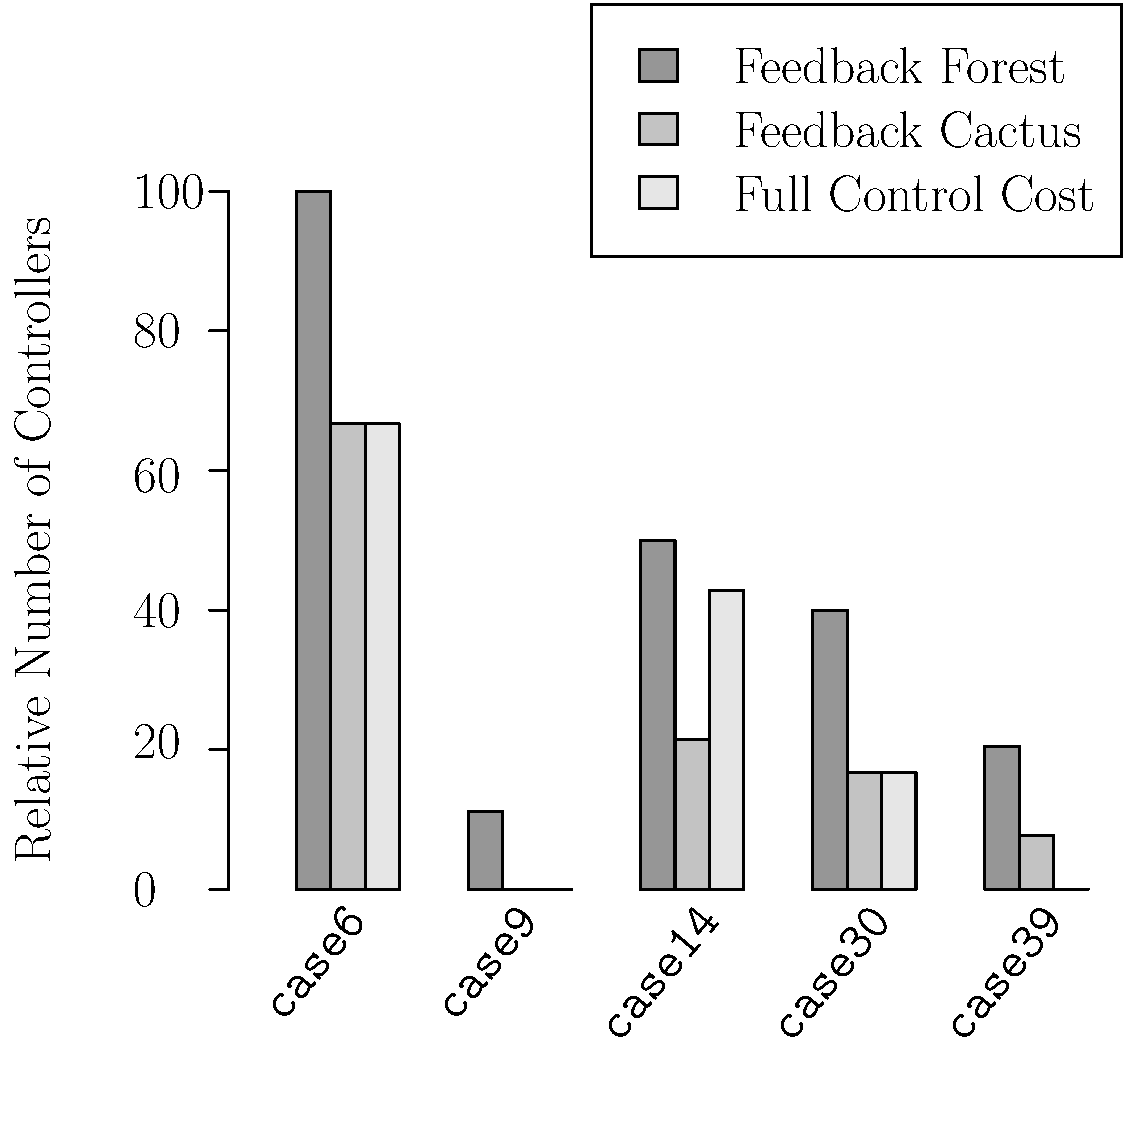
\includegraphics[width=\textwidth, page=1, trim=0cm 1.5cm 0cm 0cm]{factsplacement/figures/plotBarchartCasesVsController.pdf}
        \caption{}
        \label{ch:facts:fig:structural-results}
    \end{subfigure}%
    \caption[Minimum number of controllers to reach full control.]{
    (a) \gls{ieee} benchmark \texttt{case14} including the minimum numbers of
            controllers for \mbox{$\lambda = 0.5$}, where the bold normal lines
            represent~$\glssymbol{graph}-\glssymbol{factsbranch}$ and the bold
            dashed lines represent \gls{fce}s~$\glssymbol{factsbranch}$.
    (b) Comparing of the minimum feedback set sizes for forests and
        cacti with the necessary number of \gls{fce}s for full control.
        Cases 9 and 39 need zero \gls{fce}s, which is equivalent
        to~\cref{ch:facts:fig:barchart-cases-controller}.
    }
\end{figure}
% 
In this section, we transfer our previous theoretical
results from~\cref{ch:facts:sub:hybridtheory} to \gls{fce}s. Thereby, we answer
Question~\ref{ch:facts:quest:main1}: How many \gls{fce}s are necessary to
achieve the lower bound for the operation cost, which happens in case each line
is a \gls{fce}. We call this operation cost a \emph{full control cost}.

In~\cref{ch:facts:fig:graph-subgrids} the graph of the~\gls{ieee}
\texttt{case14} with the different subgrids is shown for the placement of
\gls{fce}s, that induces the operation cost equal to the full control cost. We
observe that the subgrid~$\glssymbol{graph}-\glssymbol{factsbranch}^c$
(graph~\glssymbol{graph} where the edges of~\glssymbol{factsbranch} are removed)
forms a \emph{cactus} (\ie, $c = 3$; graph where each edge lies in at most one
cycle). In other examples, we observed
that~$\glssymbol{graph}-\glssymbol{factsbranch}^c$ can be even simpler, forming
a \emph{forest} (\ie, $c = 2$; a graph without any cycle). If
$\glssymbol{graph}-\glssymbol{factsbranch}^c$ is a cactus (resp. forest)
and~$\glssymbol{factsbranch}^c$ is the smallest such set,
set~$\glssymbol{factsbranch}^c$ is called \emph{minimum diamond \emph{(resp.}
forest\emph{)} hitting set}.

In our experiments, summarized in~\cref{ch:facts:fig:structural-results}, we
compared the number of \gls{fce}s necessary for achieving the full control cost
to the size of minimum forest and diamond hitting sets. In
\texttt{case6}-\texttt{case30} the number of edges for the full control cost is
between the minimum size of a forest hitting set and that of a diamond hitting
set. In addition, \texttt{case6}, \texttt{case9} and \texttt{case30} achieve
full control cost with \gls{fce} size equal to the size of a diamond hitting
set. For \texttt{case39}, full control is achieved with fewer \gls{fce}s than
the diamond hitting set size. Unfortunately computing the optimal number of
\gls{fce}s for the larger~\gls{ieee} test cases is prohibitively
expensive with our current integer linear programming formulation.

The following two theorems provide theoretical evidence for our empirical
observations. They explain why the number of \gls{fce}s to achieve full
control cost and the size of minimum diamond/forest hitting set are related.
This relation and the fact that power grids are not dense networks, \ie, their
forest hitting set is not large, suggests that the relatively small number of
\gls{fce}s are enough to achieve the full control cost. \textcite{6507352}
give similar structural results on spanning trees, but using a different model.
% 
\begin{theorem}
    Let~$\glssymbol{graph}-\glssymbol{factsbranch}^c$ be a forest (\ie, $c =
    2$). Then every flow~\glssymbol{flow} is a feasible electrical flow
    on~$\glssymbol{graph}_{\ffactsbranch{2}}$.
\end{theorem}
% 
\begin{theorem}
    Let~$\glssymbol{graph}_{\glssymbol{factsbranch}^c}$ be a power grid with
    \gls{fce}s at the edges in~$\glssymbol{factsbranch}^c$ such
    that~$\glssymbol{graph}-\glssymbol{factsbranch}^c$ is a cactus (\ie, $c =
    3$) and every edge of~$\glssymbol{graph}-\ffactsbranch{3}$ that lies on a
    cycle has infinite line limits (or suitably bounded,
    see~\cref{ch:facts:eq:delta-for-cacti}). For any flow~\glssymbol{flow} there
    exists a flow~$\glssymbol{flow}'$ with identical cost that is electrically
    feasible for~$\glssymbol{graph}_{\glssymbol{factsbranch}}$.
\end{theorem}
% 
The proofs for these theorems can be directly derived
from~\cref{ch:facts:sub:hybridtheory} by replacing the set of flow control
vertices~$\glssymbol{factsbus}^c$ with the set of flow control
edges~$\glssymbol{factsbranch}^c$.
%
\begin{figure}[tbp!]%
    \centering
    \begin{subfigure}[t]{.492\textwidth}
        \centering
%       trim = left, bottom, right, top
        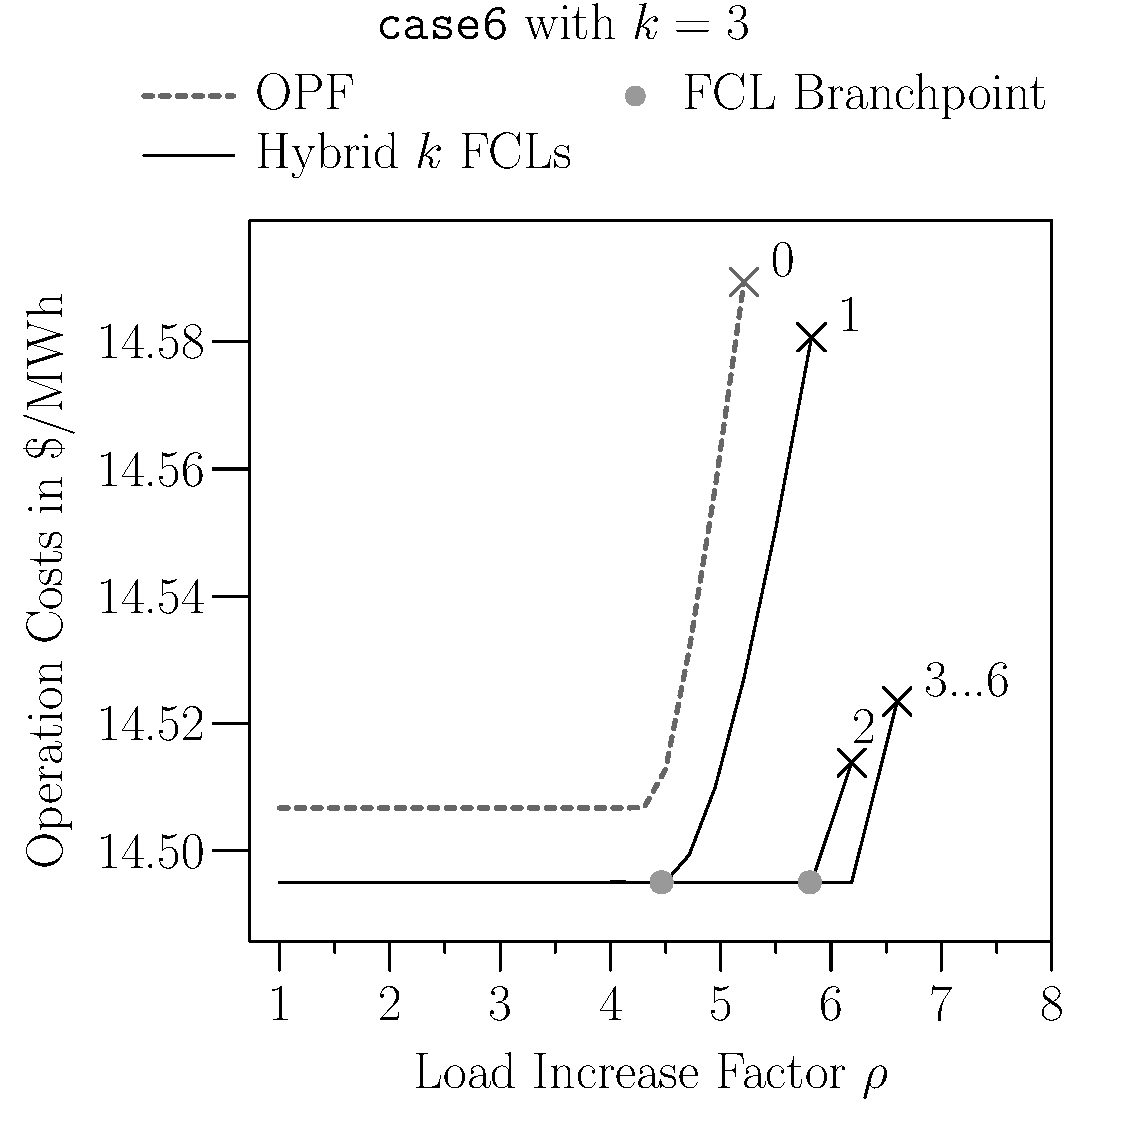
\includegraphics[width=\textwidth, page=1, trim=0cm 0cm 0cm 0cm]{factsplacement/figures/plotCapacityReductionVsCostsController.pdf}
    \end{subfigure}
%
    \hfill
    \begin{subfigure}[t]{.492\textwidth}
        \centering
%       trim = left, bottom, right, top
        \includegraphics[width=\textwidth, page=2, trim=0cm 0cm 0cm 0cm]{factsplacement/figures/plotCapacityReductionVsCostsController.pdf}
    \end{subfigure}
    
    \vspace*{0.5cm}
    \begin{subfigure}[t]{.492\textwidth}
        \centering
%       trim = left, bottom, right, top
        \includegraphics[width=\textwidth, page=3, trim=0cm 0cm 0cm 0cm]{factsplacement/figures/plotCapacityReductionVsCostsController.pdf}
    \end{subfigure}
%
    \hfill
    \begin{subfigure}[t]{.492\textwidth}
        \centering
%       trim = left, bottom, right, top
        \includegraphics[width=\textwidth, page=4, trim=0cm 0cm 0cm 0cm]{factsplacement/figures/plotCapacityReductionVsCostsController.pdf}
    \end{subfigure}
    
    \vspace*{0.5cm}
    \begin{subfigure}[t]{.492\textwidth}
        \centering
%       trim = left, bottom, right, top
        \includegraphics[width=\textwidth, page=5, trim=0cm 0cm 0cm 0cm]
        {factsplacement/figures/plotCapacityReductionVsCostsController.pdf}
    \end{subfigure}
%
    \hfill
    \begin{subfigure}[t]{.492\textwidth}
        \centering
%       trim = left, bottom, right, top
        \includegraphics[width=\textwidth, page=6, trim=0cm 0cm 0cm 0cm]{factsplacement/figures/plotCapacityReductionVsCostsController.pdf}
    \end{subfigure}
    % 
    \caption[Overview of operation costs while placing~\gls{facts}.]
    {Overview of operation costs for~\texttt{case6} to~\texttt{case57}
    for~\gls{opfp} ($0$~\gls{fce}s) and the hybrid model with respect
    to load increase factor~$\rho$, where~$k$ is the upper bound
    for~\gls{fce}s. The numbers on the curves represent the number
    of~\gls{fce}s for that specific curve. Cases 9 and 39 need
    zero~\gls{fce}s, equivalent to the results for~\gls{fcv}s.}
    \label{ch:facts:figure:appendix}
\end{figure}
%
%%%%%%%%%%%%%%%%%%%%%%%%%%%%%%%%%%%%%%%%%%%%%%%%%%%%%%%%%%%%%%%%%%%%%%%%%%%%%%%%
\section{Effect of FCEs in Comparision to FCVs}
\label{ch:facts-branches:sec:effect-of-fcls-in-comparison-to-FCBs}
%%%%%%%%%%%%%%%%%%%%%%%%%%%%%%%%%%%%%%%%%%%%%%%%%%%%%%%%%%%%%%%%%%%%%%%%%%%%%%%%
%
In this section we evaluate~\cref{ch:facts:quest:main2}. For this reason, we
increase the load by a factor~$\rho$ until the model becomes infeasible. For the
hybrid model this happens when adding more \gls{fce}s does not extend the
operability.

\cref{ch:facts:figure:appendix} show the experimental results for the~\gls{ieee}
power grids~\texttt{case6} to~\texttt{case57}. The behavior is the same as
for~\gls{fcv}s meaning that the operation cost and the range of operability
increase when increasing the load factor~$\rho$. Interestingly, the number
of~\gls{fce}s does not increase substantially. For the \texttt{case14} there is
a maximum of three~\gls{fce}s necessary instead of two~\gls{fcv}s and for
the~\texttt{case57} the number of maximum~\gls{fce}s remains the same as
for~\gls{fcv}s. Similar behavior can be observed for the remaining cases. Recall
that~\gls{fcv}s control flow on all incident edges, which can be realized by
placing~\gls{facts} on all of these edges. Thus, in case of~\gls{fcv}s the
number of necessary~\gls{facts} actually depends on the degree of the vertices
holding the~\gls{fcv}s and results in large number of~\gls{facts} as indicated
in~\cref{ch:facts:tab:comparison}.
%
\begin{table}[tb!]
    \centering
    % 
    \caption[Comparison of the~\gls{fcv} and~\gls{fce} Model.]
    {Comparison of the previous model using~\gls{fcv}s and the current model
    using~\gls{fce}s. To compute the number of~\gls{facts} in case
    of~\gls{fcv}s, we compute the total number of edges incident to the vertices
    holding~\gls{fcv}s.}
    % 
    \label{ch:facts:tab:comparison}
    % 
    \begin{tabular}{@{}clrrrrr@{}}
\toprule
\multicolumn{2}{c}{{\textbf{Dependency of Con-\hspace*{0.3cm}}}}
& \multicolumn{1}{c}{{\textbf \texttt{case6}}} 
& \multicolumn{1}{c}{\hspace*{0.1cm}{\textbf \texttt{case9}}} 
& \multicolumn{1}{c}{\hspace*{0.1cm}{\textbf \texttt{case14}}} 
& \multicolumn{1}{c}{\hspace*{0.1cm}{\textbf \texttt{case30}}} 
& \multicolumn{1}{c}{\hspace*{0.1cm}{\textbf \texttt{case39}}} 
\\
\multicolumn{2}{c}{{\textbf{trol Units Number\hspace*{0.3cm}}}}
& \multicolumn{1}{c}{{\textbf \texttt{}}} 
& \multicolumn{1}{c}{\hspace*{0.1cm}{\textbf \texttt{}}} 
& \multicolumn{1}{c}{\hspace*{0.1cm}{\textbf \texttt{}}} 
& \multicolumn{1}{c}{\hspace*{0.1cm}{\textbf \texttt{}}} 
& \multicolumn{1}{c}{\hspace*{0.1cm}{\textbf \texttt{}}} 
\\ 
\midrule
\multirow{3}{*}{\acrshort{fce}s\hspace*{0.2cm}} 
& Feedback Edge Set        
& 6  
& 1                                   
& 7                                 
& 12                               
& 8  
\\
& Diamond Hitting Set    
& 4                             
& 0 
& 3
& 5
& 3
\\
& Full Control
& 4
& 0
& 6
& 5
& 0
\\ \midrule
\multirow{6}{*}{\acrshort{fcv}s\hspace*{0.2cm}} 
& Feedback Edge Set
& 2
& 1
& 3
& 5
& 4
\\
& \acrshort{facts}
& 9
& 2
& 11
& 21
& 15
\\ \cmidrule(l){2-7} 
& Diamond Hitting Set
& 1
& 0
& 2
& 2
& 2
\\
& \acrshort{facts}
& 5
& 0
& 8
& 10
& 5
\\ \cmidrule(l){2-7} 
& Full Control
& 2
& 1
& 2
& 5
& 4
\\
& \acrshort{facts}
& 9
& 3
& 8
& 23
& 15
\\ \bottomrule
\end{tabular}
\end{table}
%
%%%%%%%%%%%%%%%%%%%%%%%%%%%%%%%%%%%%%%%%%%%%%%%%%%%%%%%%%%%%%%%%%%%%%%%%%%%%%%%%
\section{Conclusion}    
\label{facts:sec:conclusion}
%%%%%%%%%%%%%%%%%%%%%%%%%%%%%%%%%%%%%%%%%%%%%%%%%%%%%%%%%%%%%%%%%%%%%%%%%%%%%%%%
%
Assuming the existence of special vertices that control the flow on all their
incident transmission lines, we have presented a hybrid model for including some
flow control vertices.  In this model, we have shown that relatively few control
vertices suffice for achieving full control. Further, we scaled the load of the
network and showed that even fewer flow control vertices improve the loadability
and have a lower cost increase compared to~\gls{opf}. 

A more realistic assumption is the placement of flow control units on edges,
which we call~\gls{fce}s. Here, we were able to transfer the results of~\gls{fcv}s and
make some similar observations.

Our work shows the benefits of augmenting power grids with flow control devices.
Using our theoretical model, we were able to explain our empirical observations
on controller placement with graph-theoretical means. While this also explains
previous observations of~\textcite{gcg-olmtf-01}, the main drawback is that the
model is based on several strong, simplifying assumptions such as neglecting
line losses.

% Future work should consider more realistic power grid models both in terms of
% the control units, which are placed on transmission lines rather than vertices,
% and using the~\gls{ac} power grid model.
%